\section{Results}

This section should provide an overview of the capabilities of the introduced 
mesh generation, adaption and classification software package.

\subsection{CMOS structure}

In the following, different views of the original and the adapted 
volume mesh are presented. Additionally, a comparison of the mesh quality 
is depicted.

\begin{figure}[!ht]
   \centering
   \subfloat%[\textsc{Initial Mesh}]
   {
      \fbox{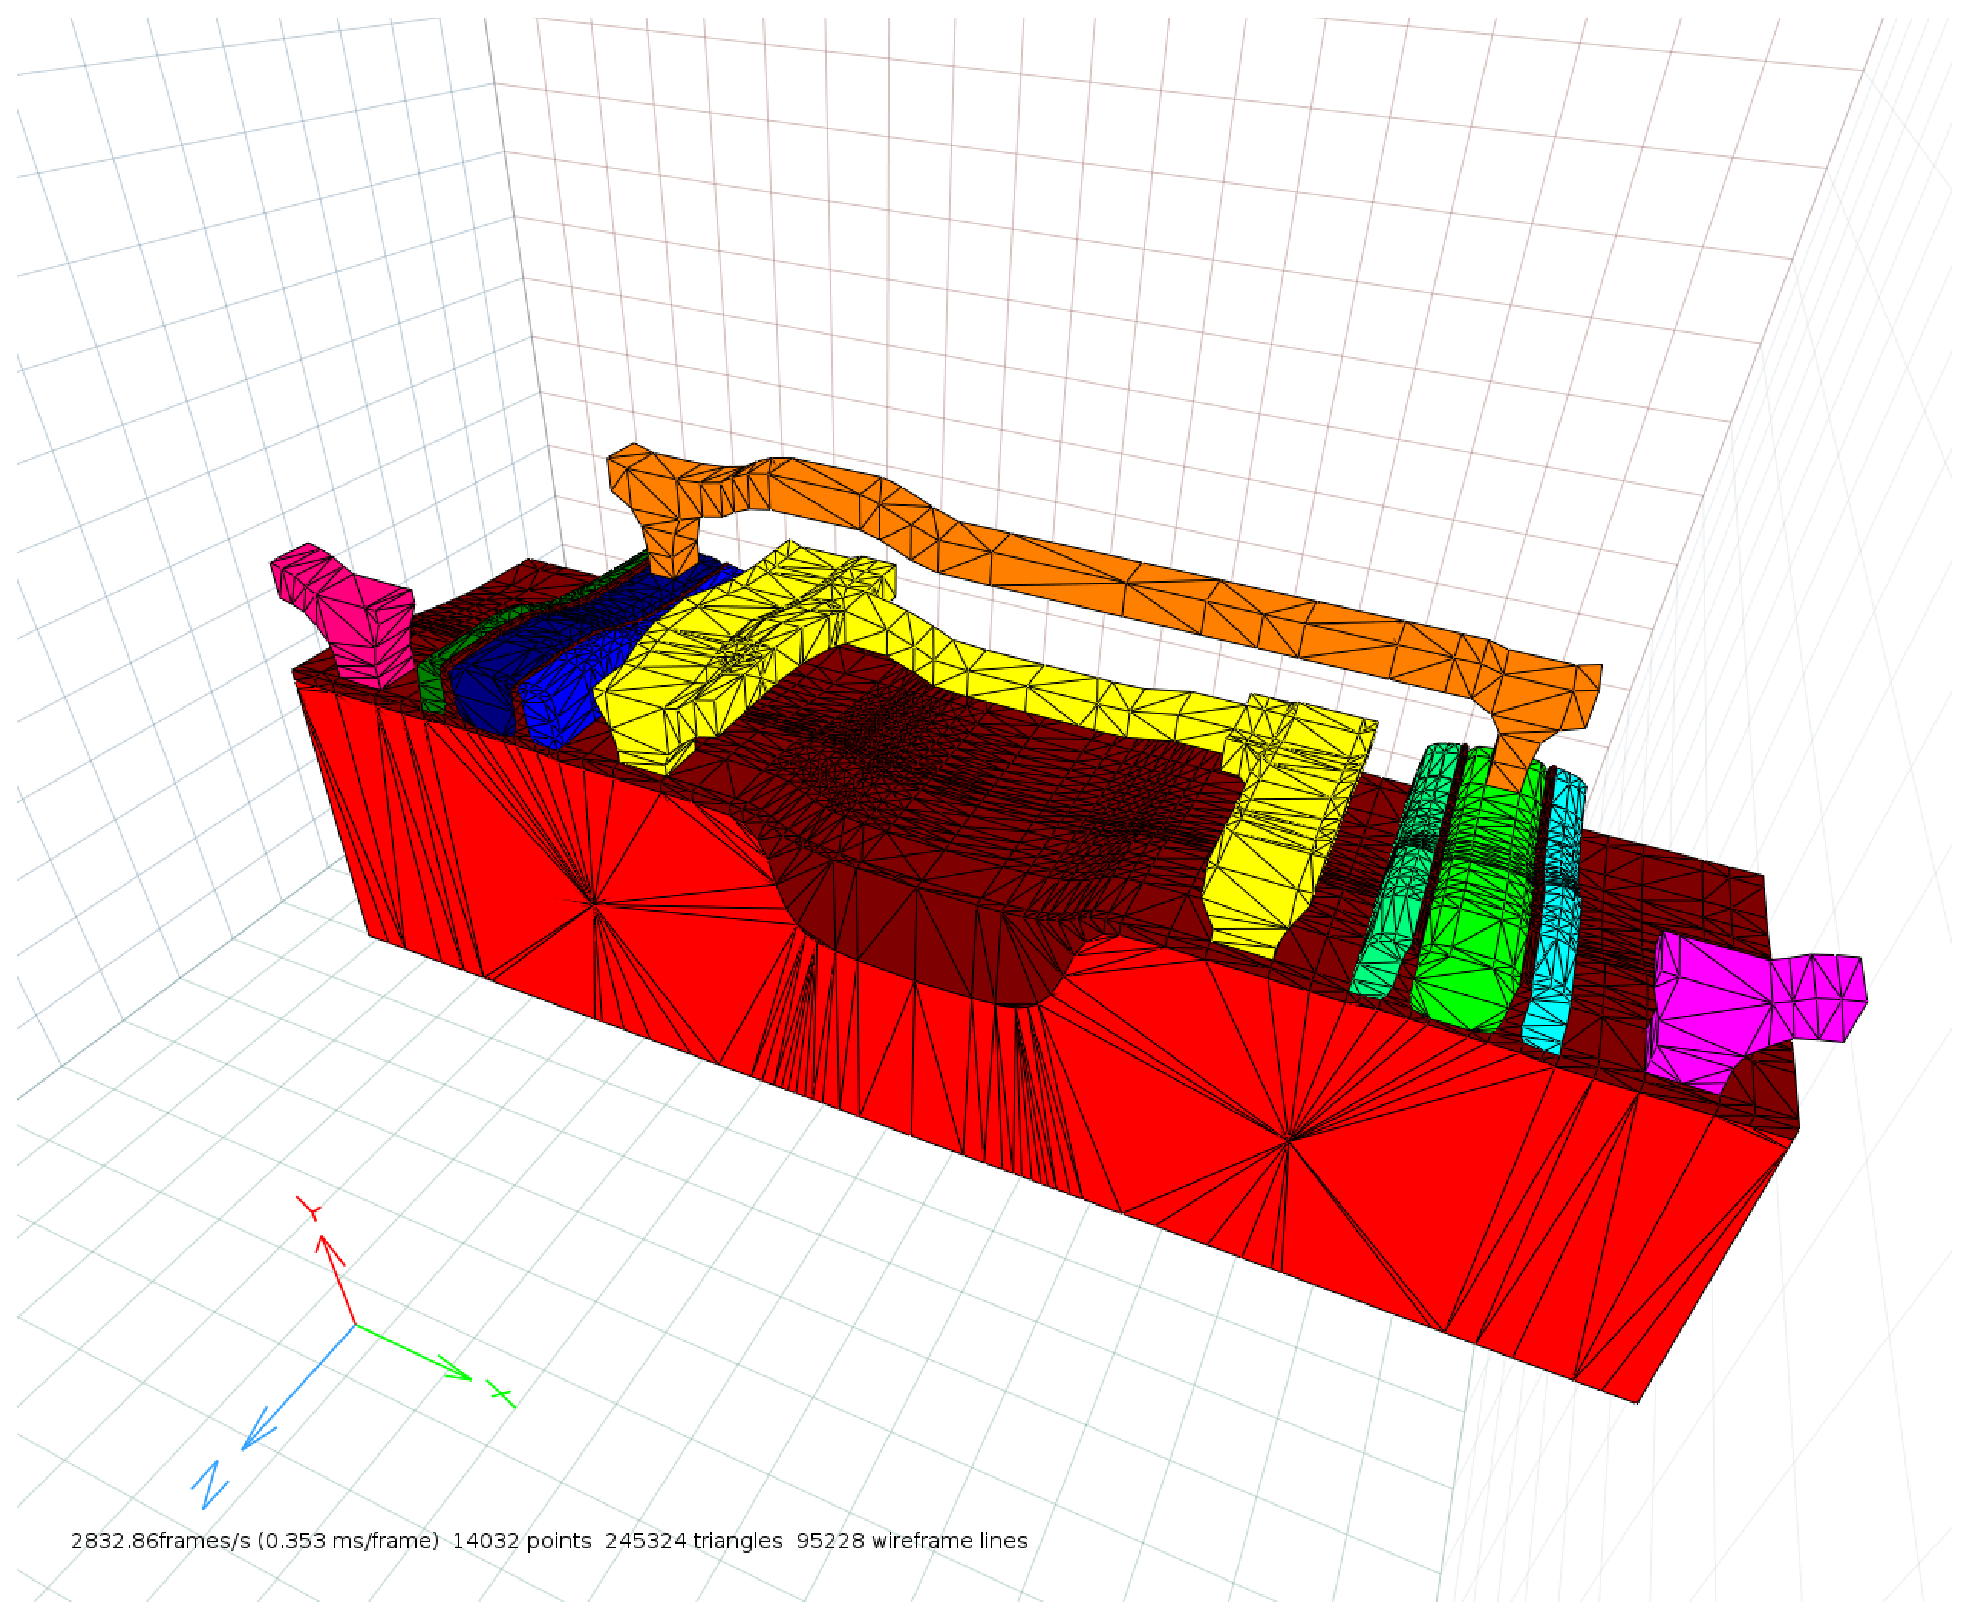
\includegraphics[scale=0.2]{figures/raw/cmos_orig_total.eps}}
   }
   \subfloat%[\textsc{Adapted Mesh}]
   {
      \fbox{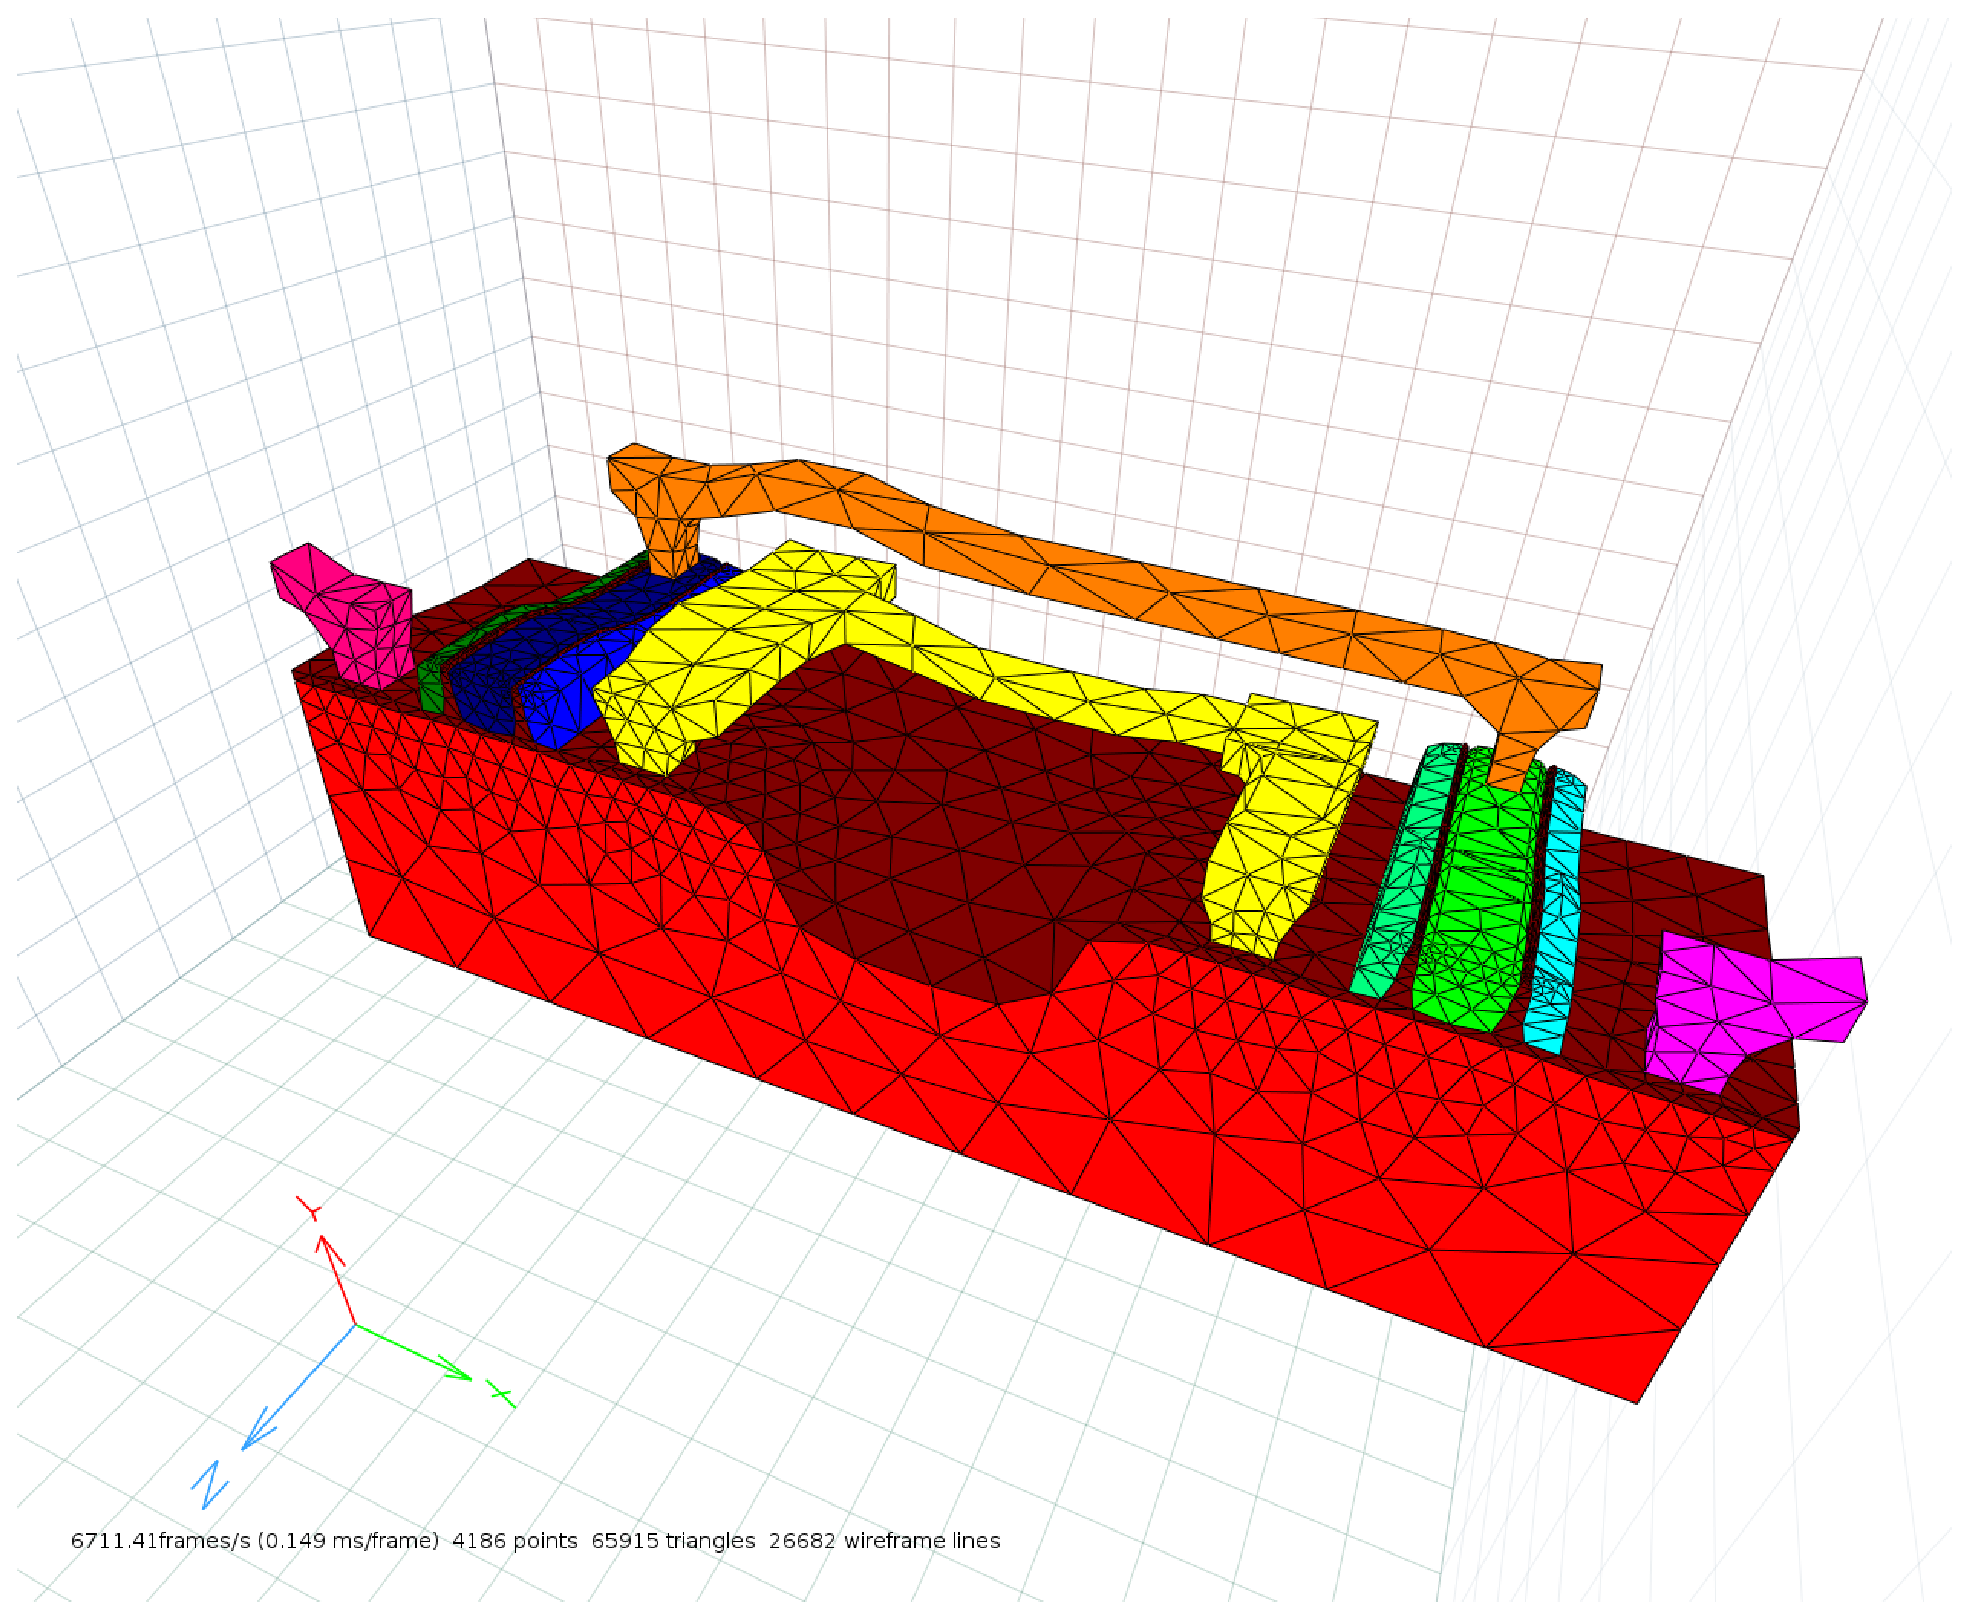
\includegraphics[scale=0.20]{figures/raw/cmos_adapted_total.eps}}
   }

   \subfloat%[\textsc{Initial Mesh}]
   {
      \fbox{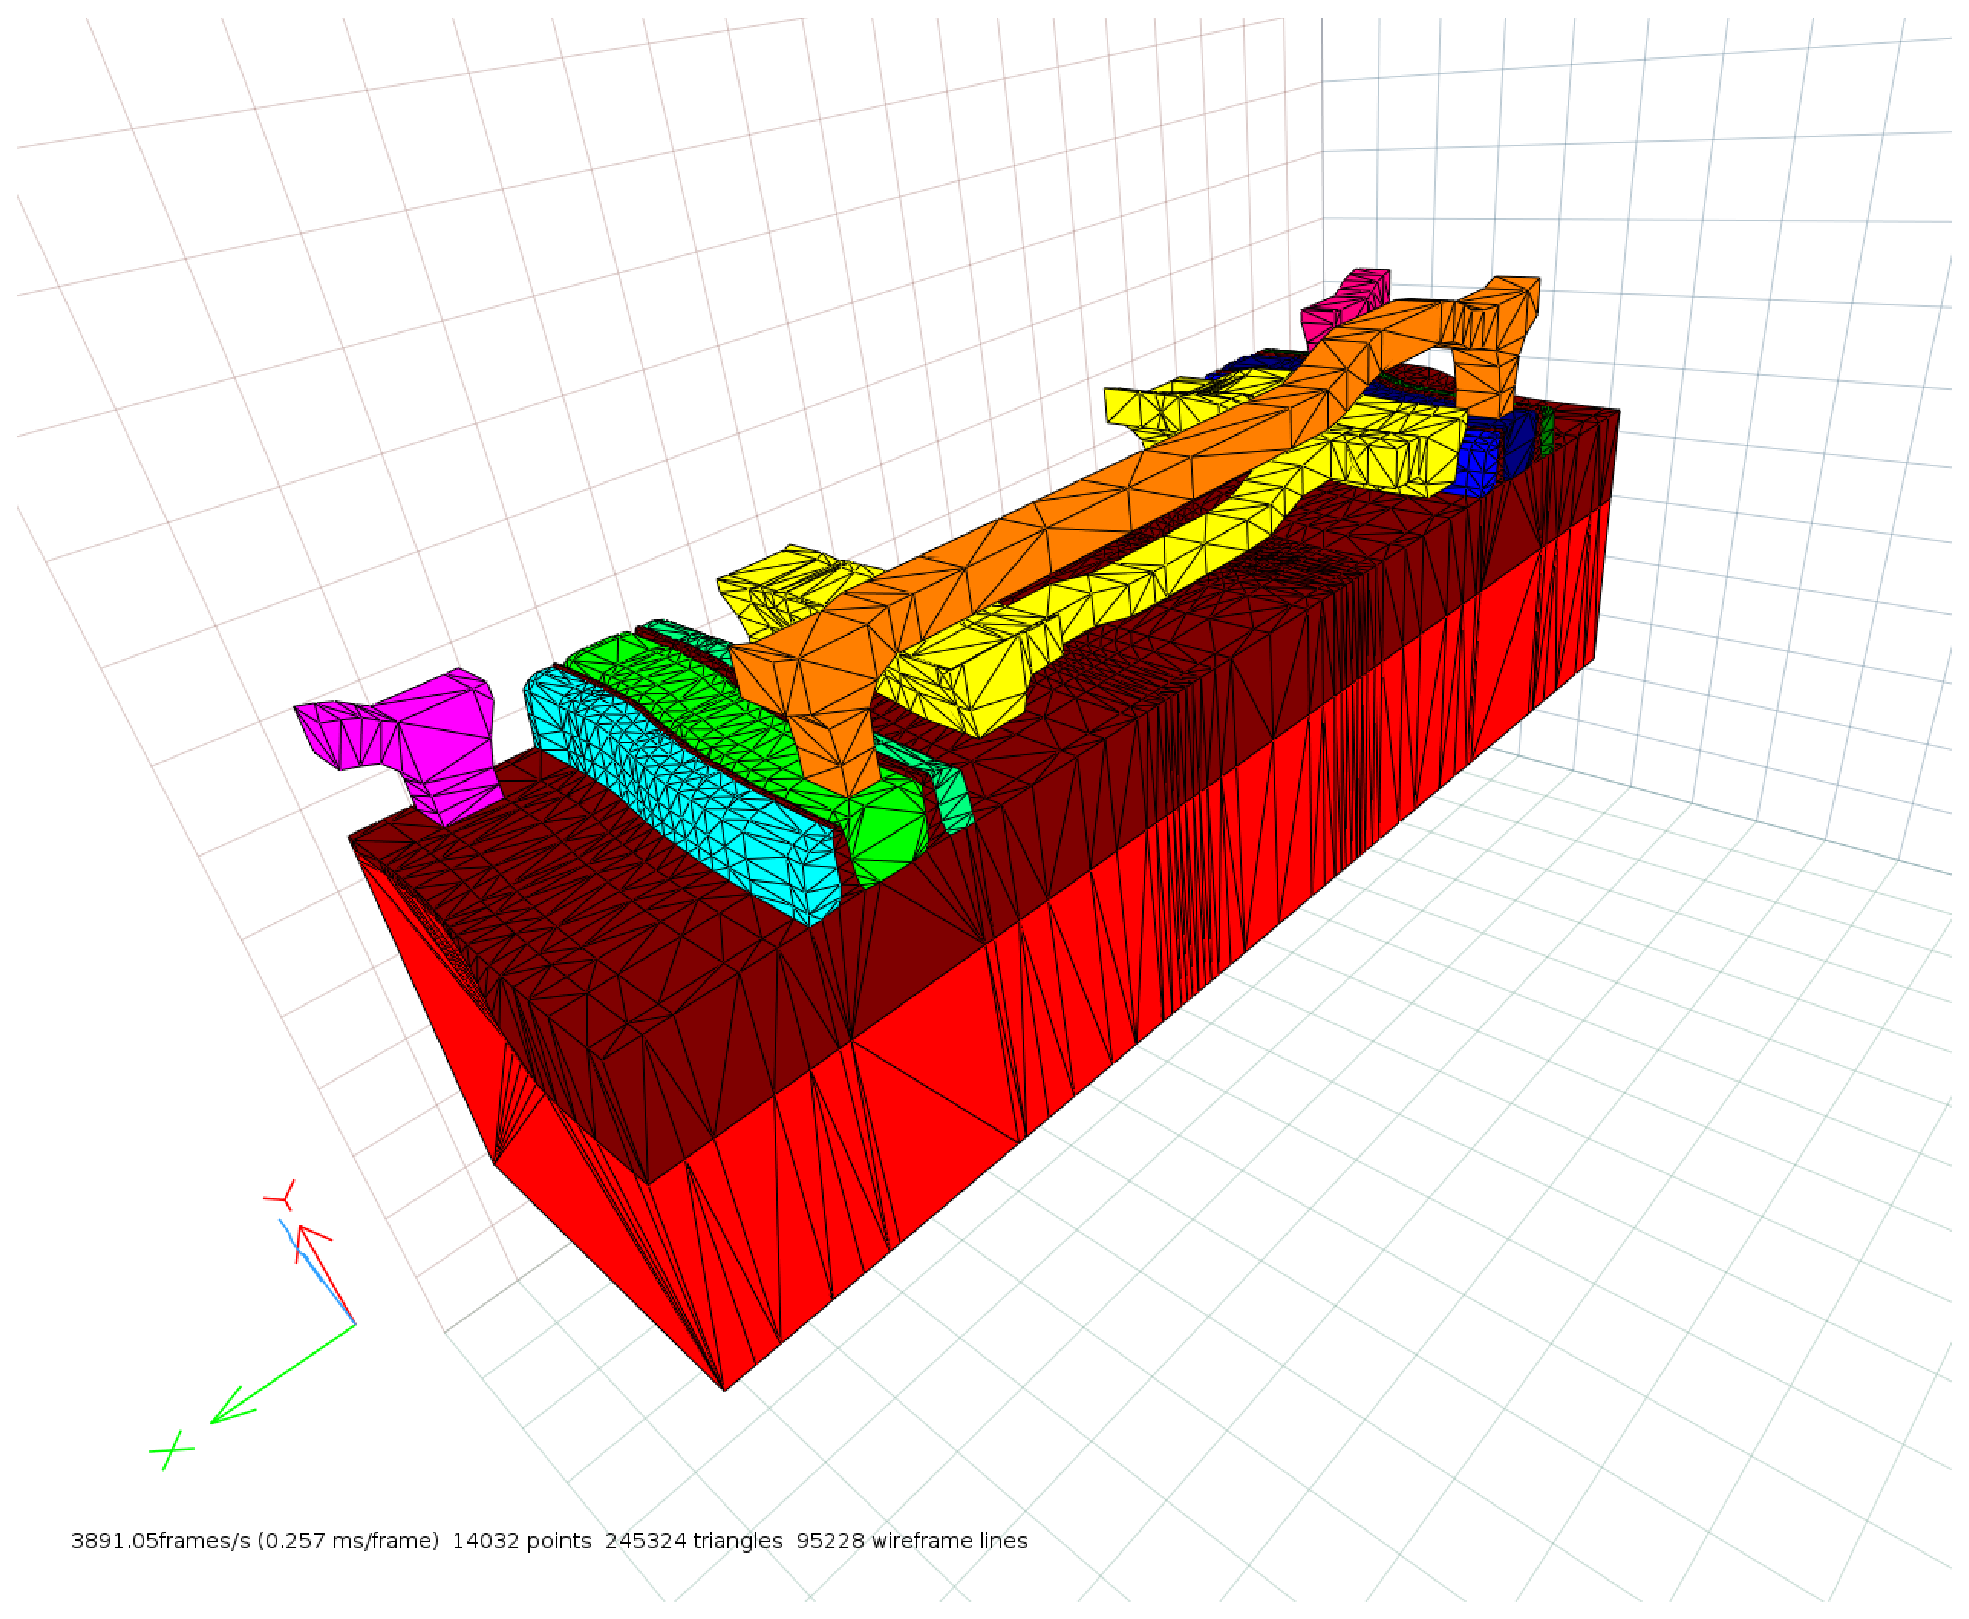
\includegraphics[scale=0.2]{figures/raw/cmos_orig_total_back.eps}}
   }
   \subfloat%[\textsc{Adapted Mesh}]
   {
      \fbox{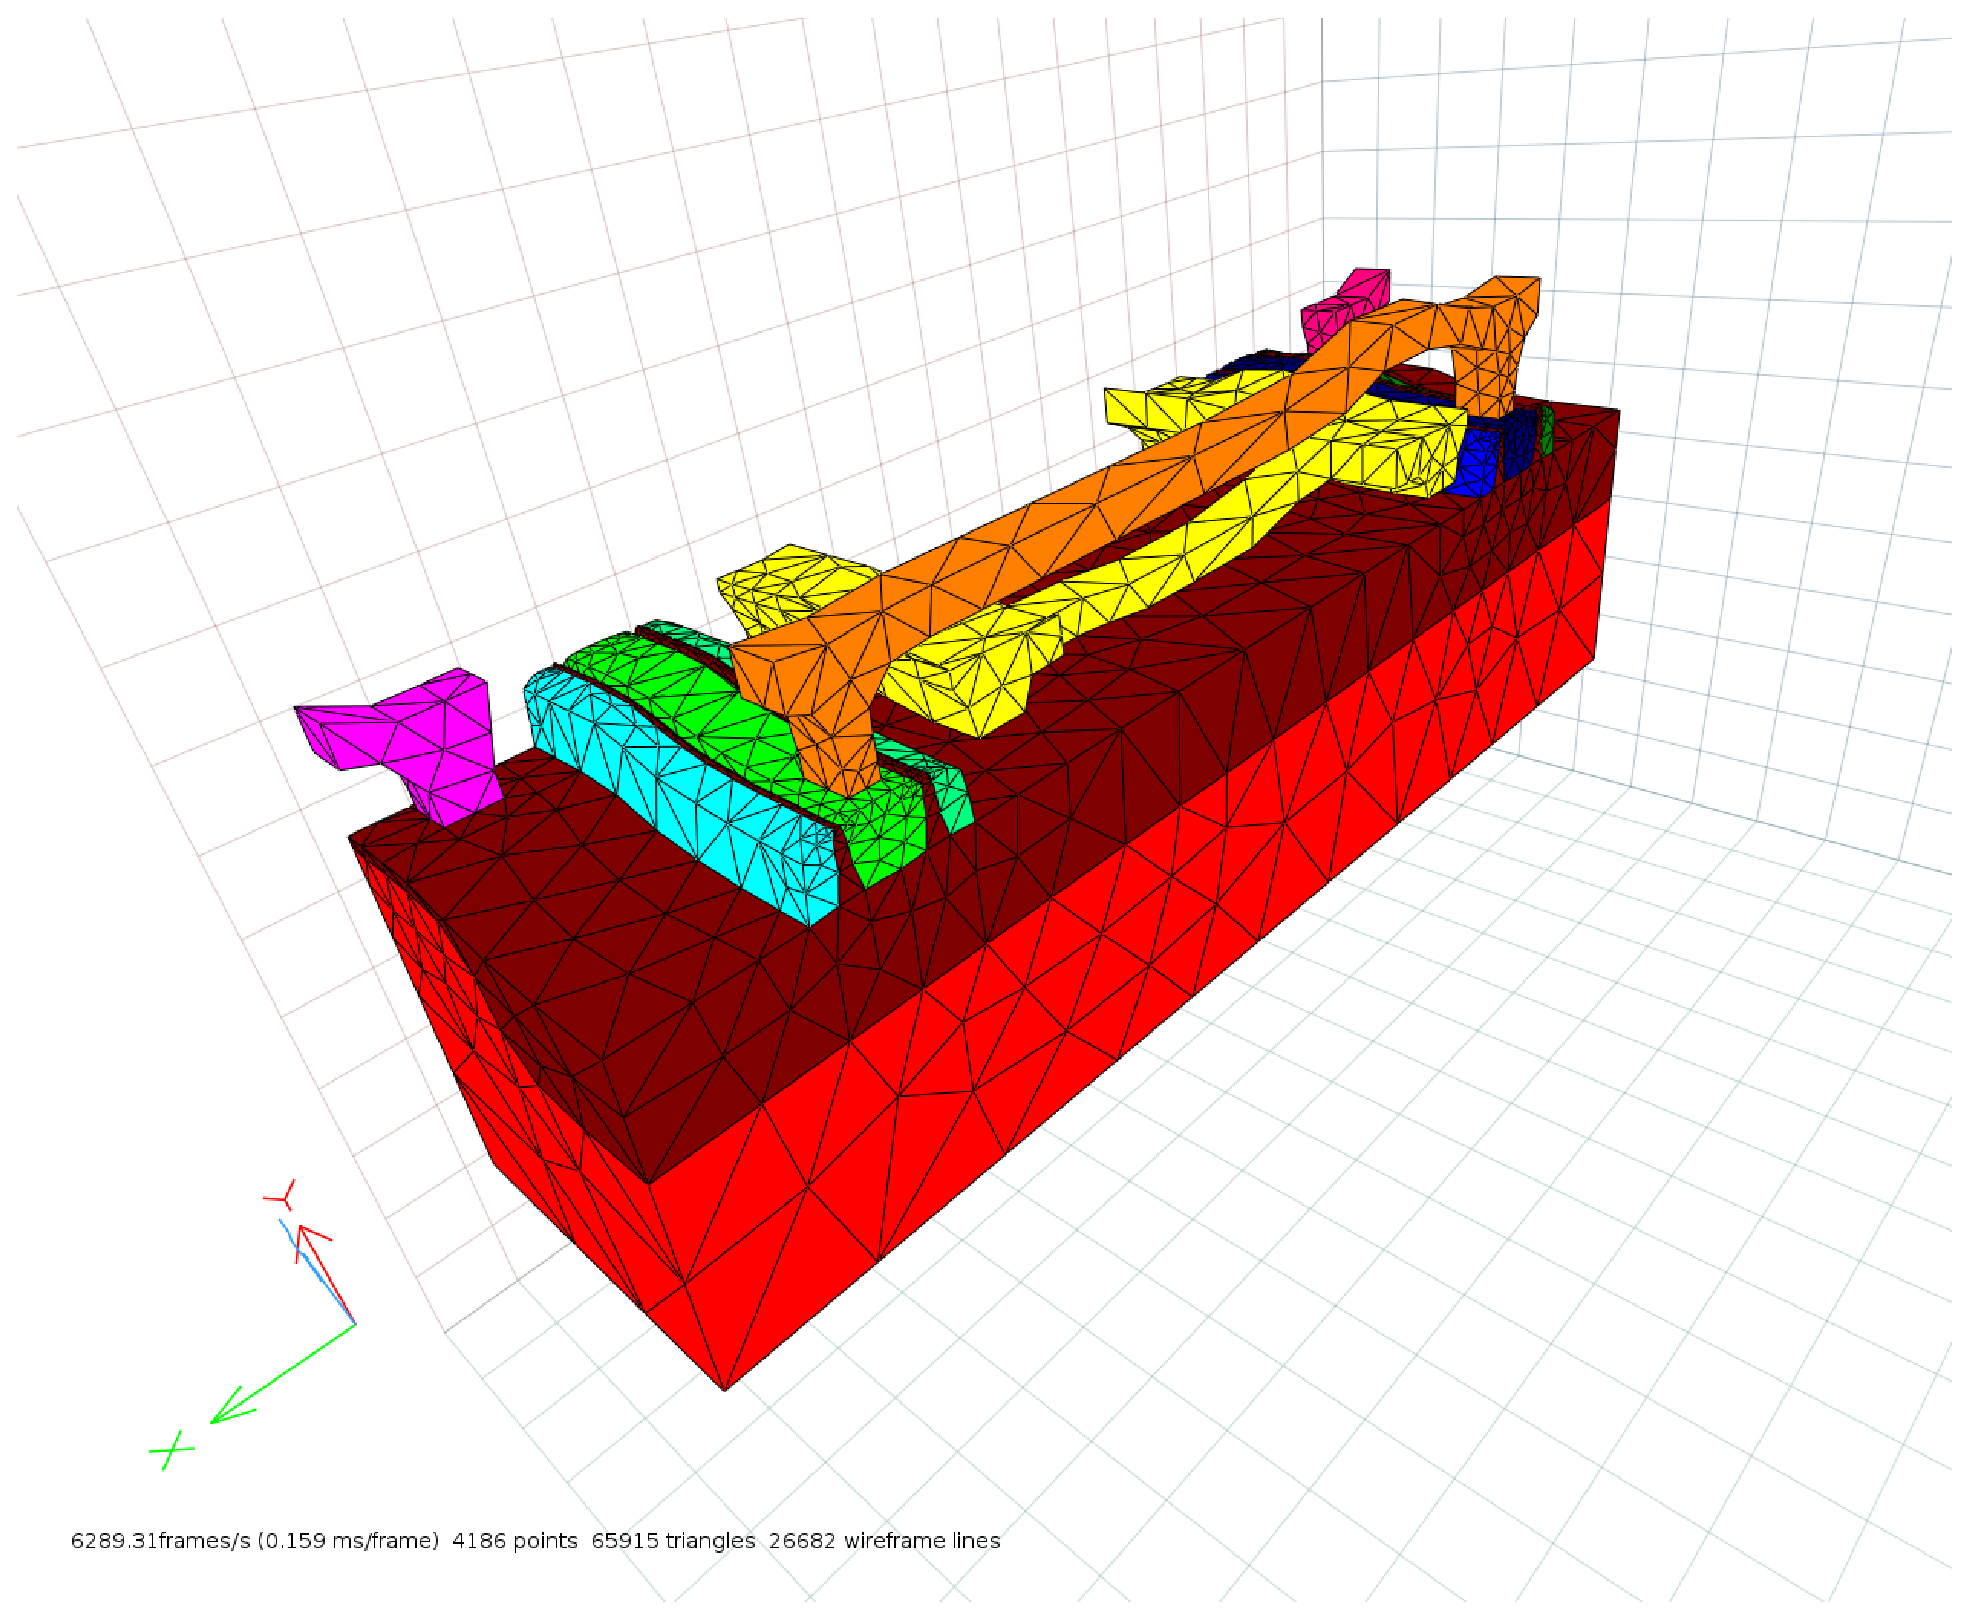
\includegraphics[scale=0.20]{figures/raw/cmos_adapted_total_back.eps}}
   }
   \caption{A CMOS structure.\newline
   \textbf{left:} The initial mesh is shown. \textbf{right:} The adapted mesh is shown. }
\end{figure}

\begin{figure}[!ht]
   \centering
   \subfloat%[\textsc{Initial Mesh}]
   {
      \fbox{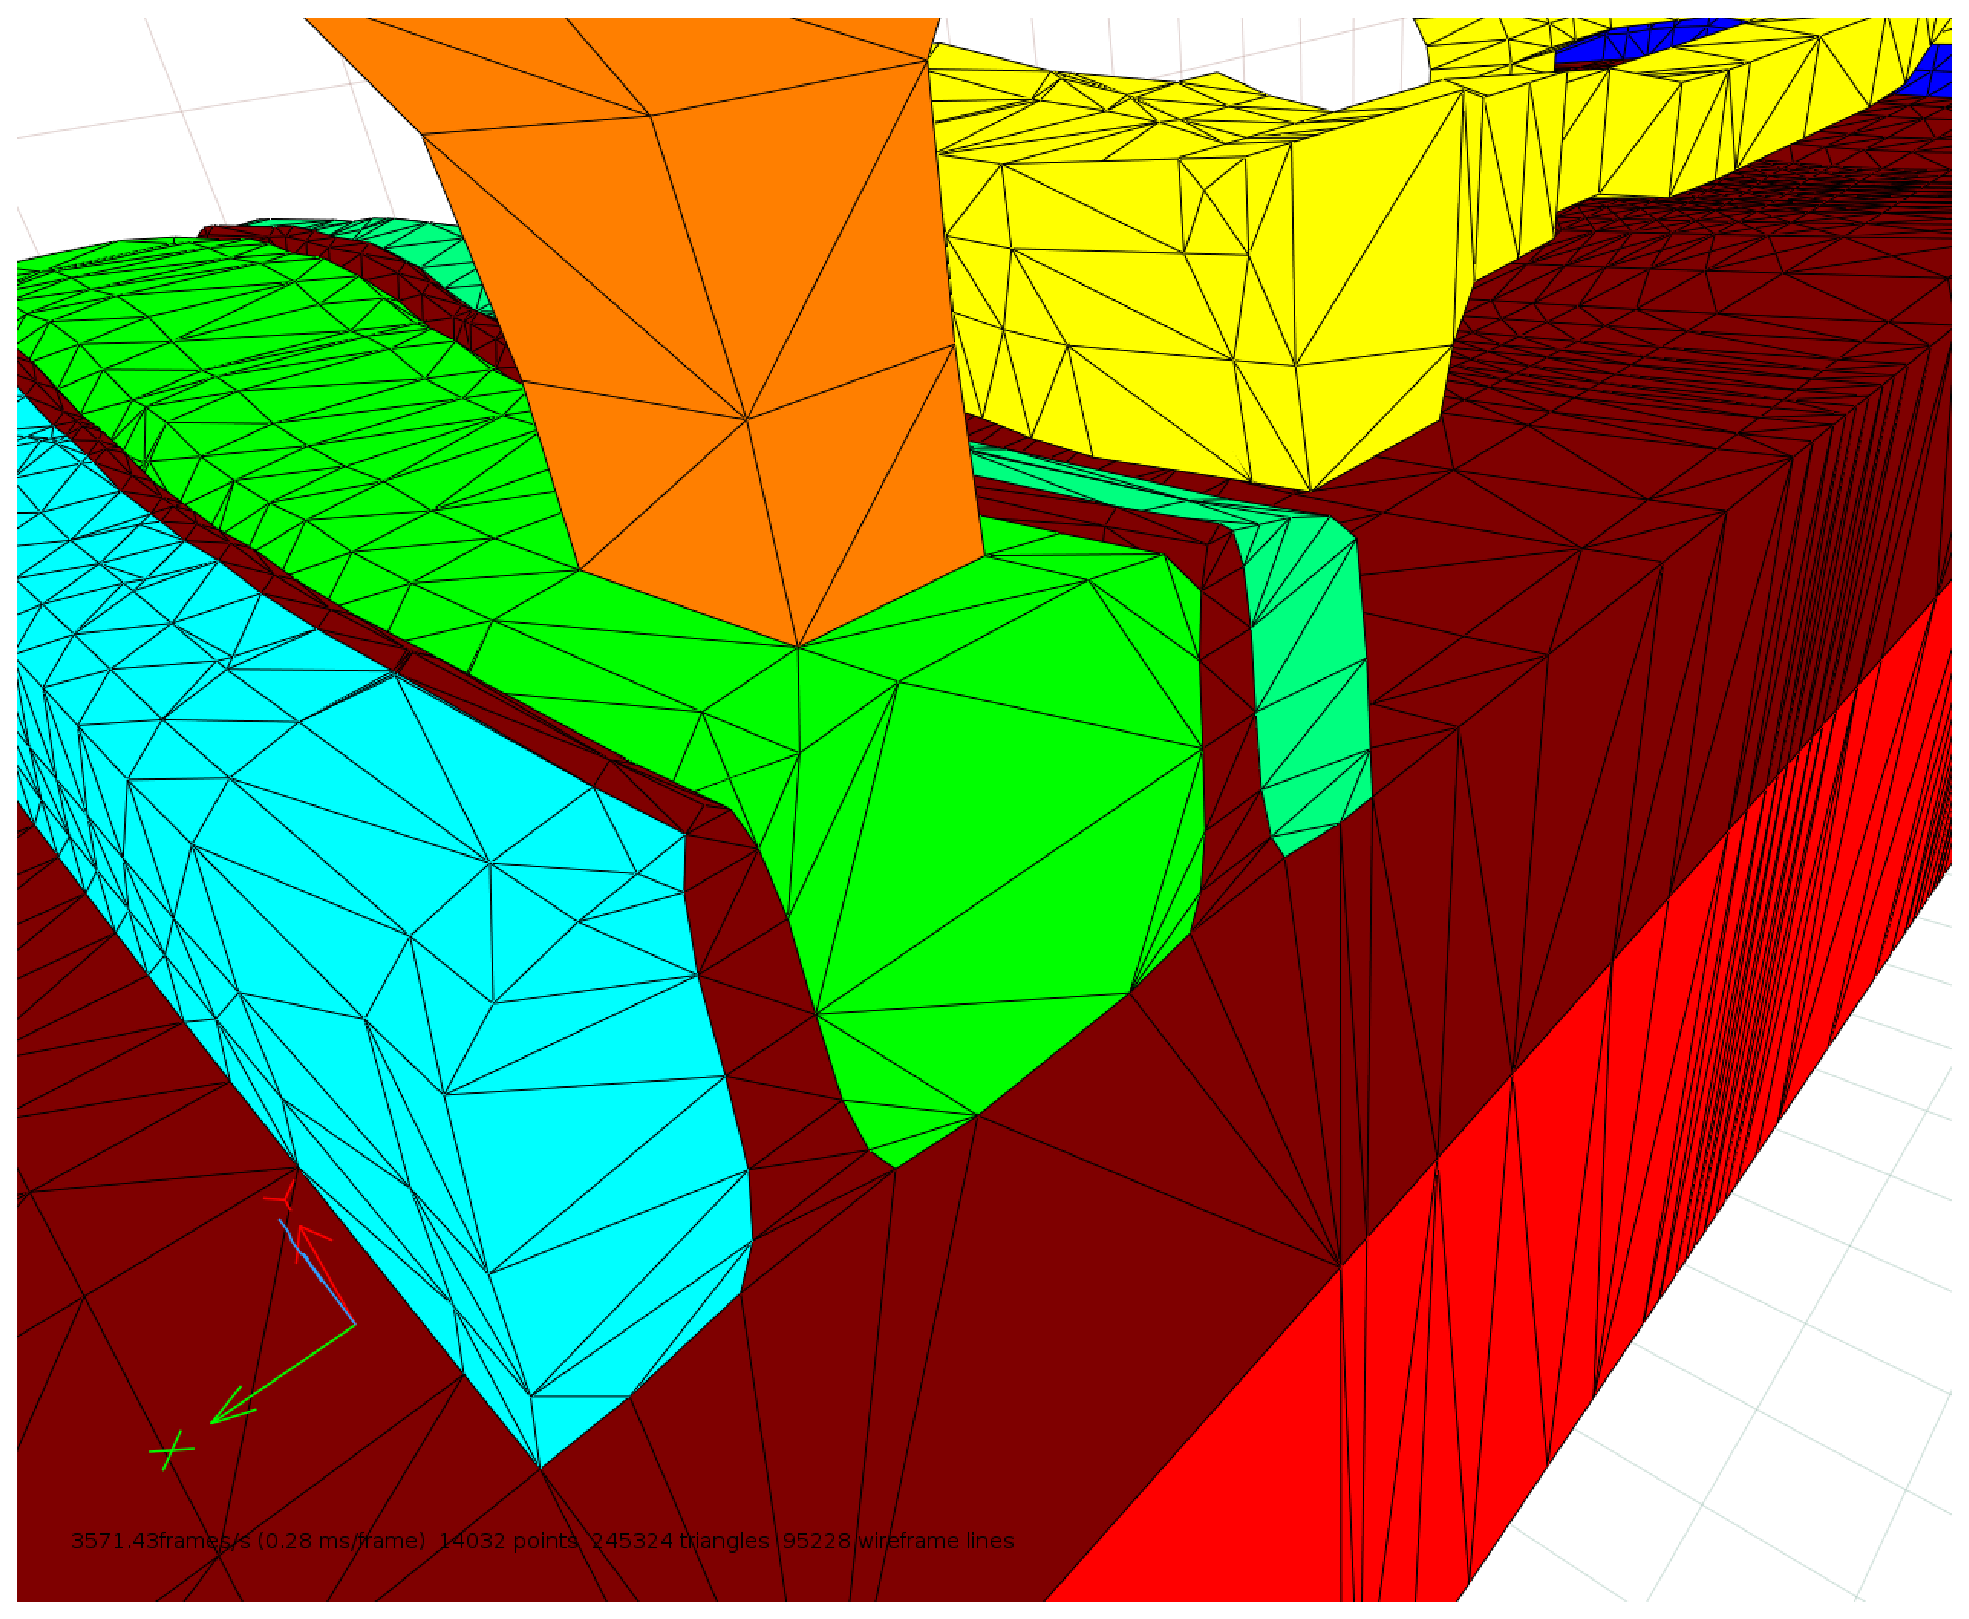
\includegraphics[scale=0.2]{figures/raw/cmos_orig_close.eps}}
   }
   \subfloat%[\textsc{Adapted Mesh}]
   {
      \fbox{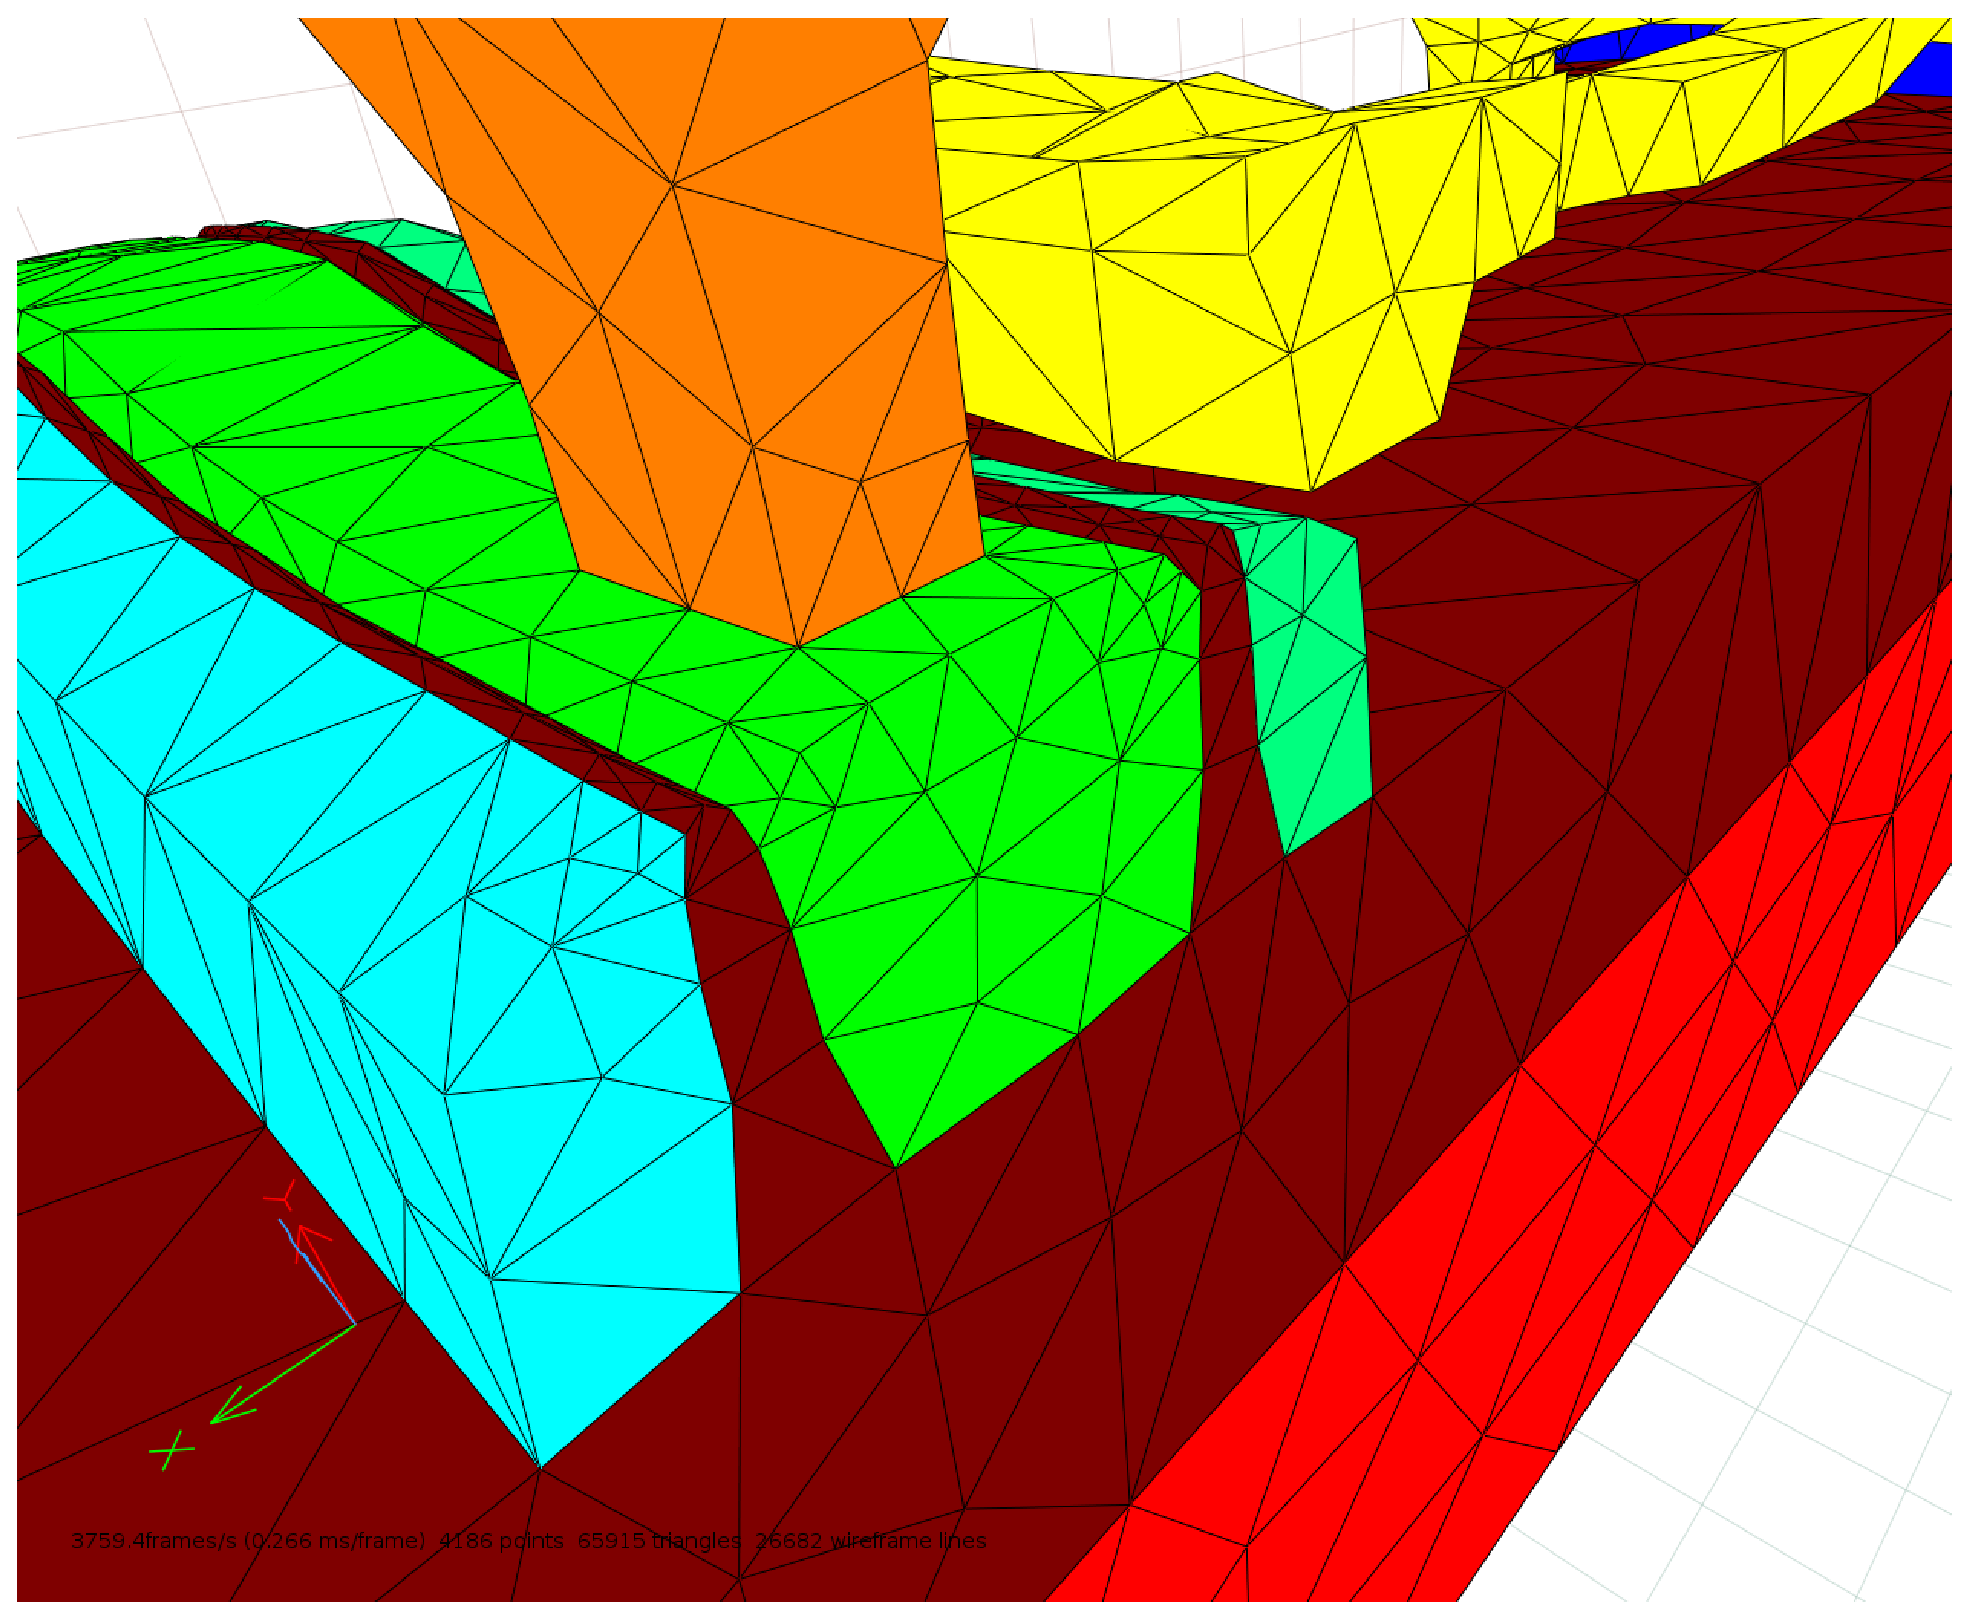
\includegraphics[scale=0.20]{figures/raw/cmos_adapted_close.eps}}
   }

   \subfloat%[\textsc{Initial Mesh}]
   {
      \fbox{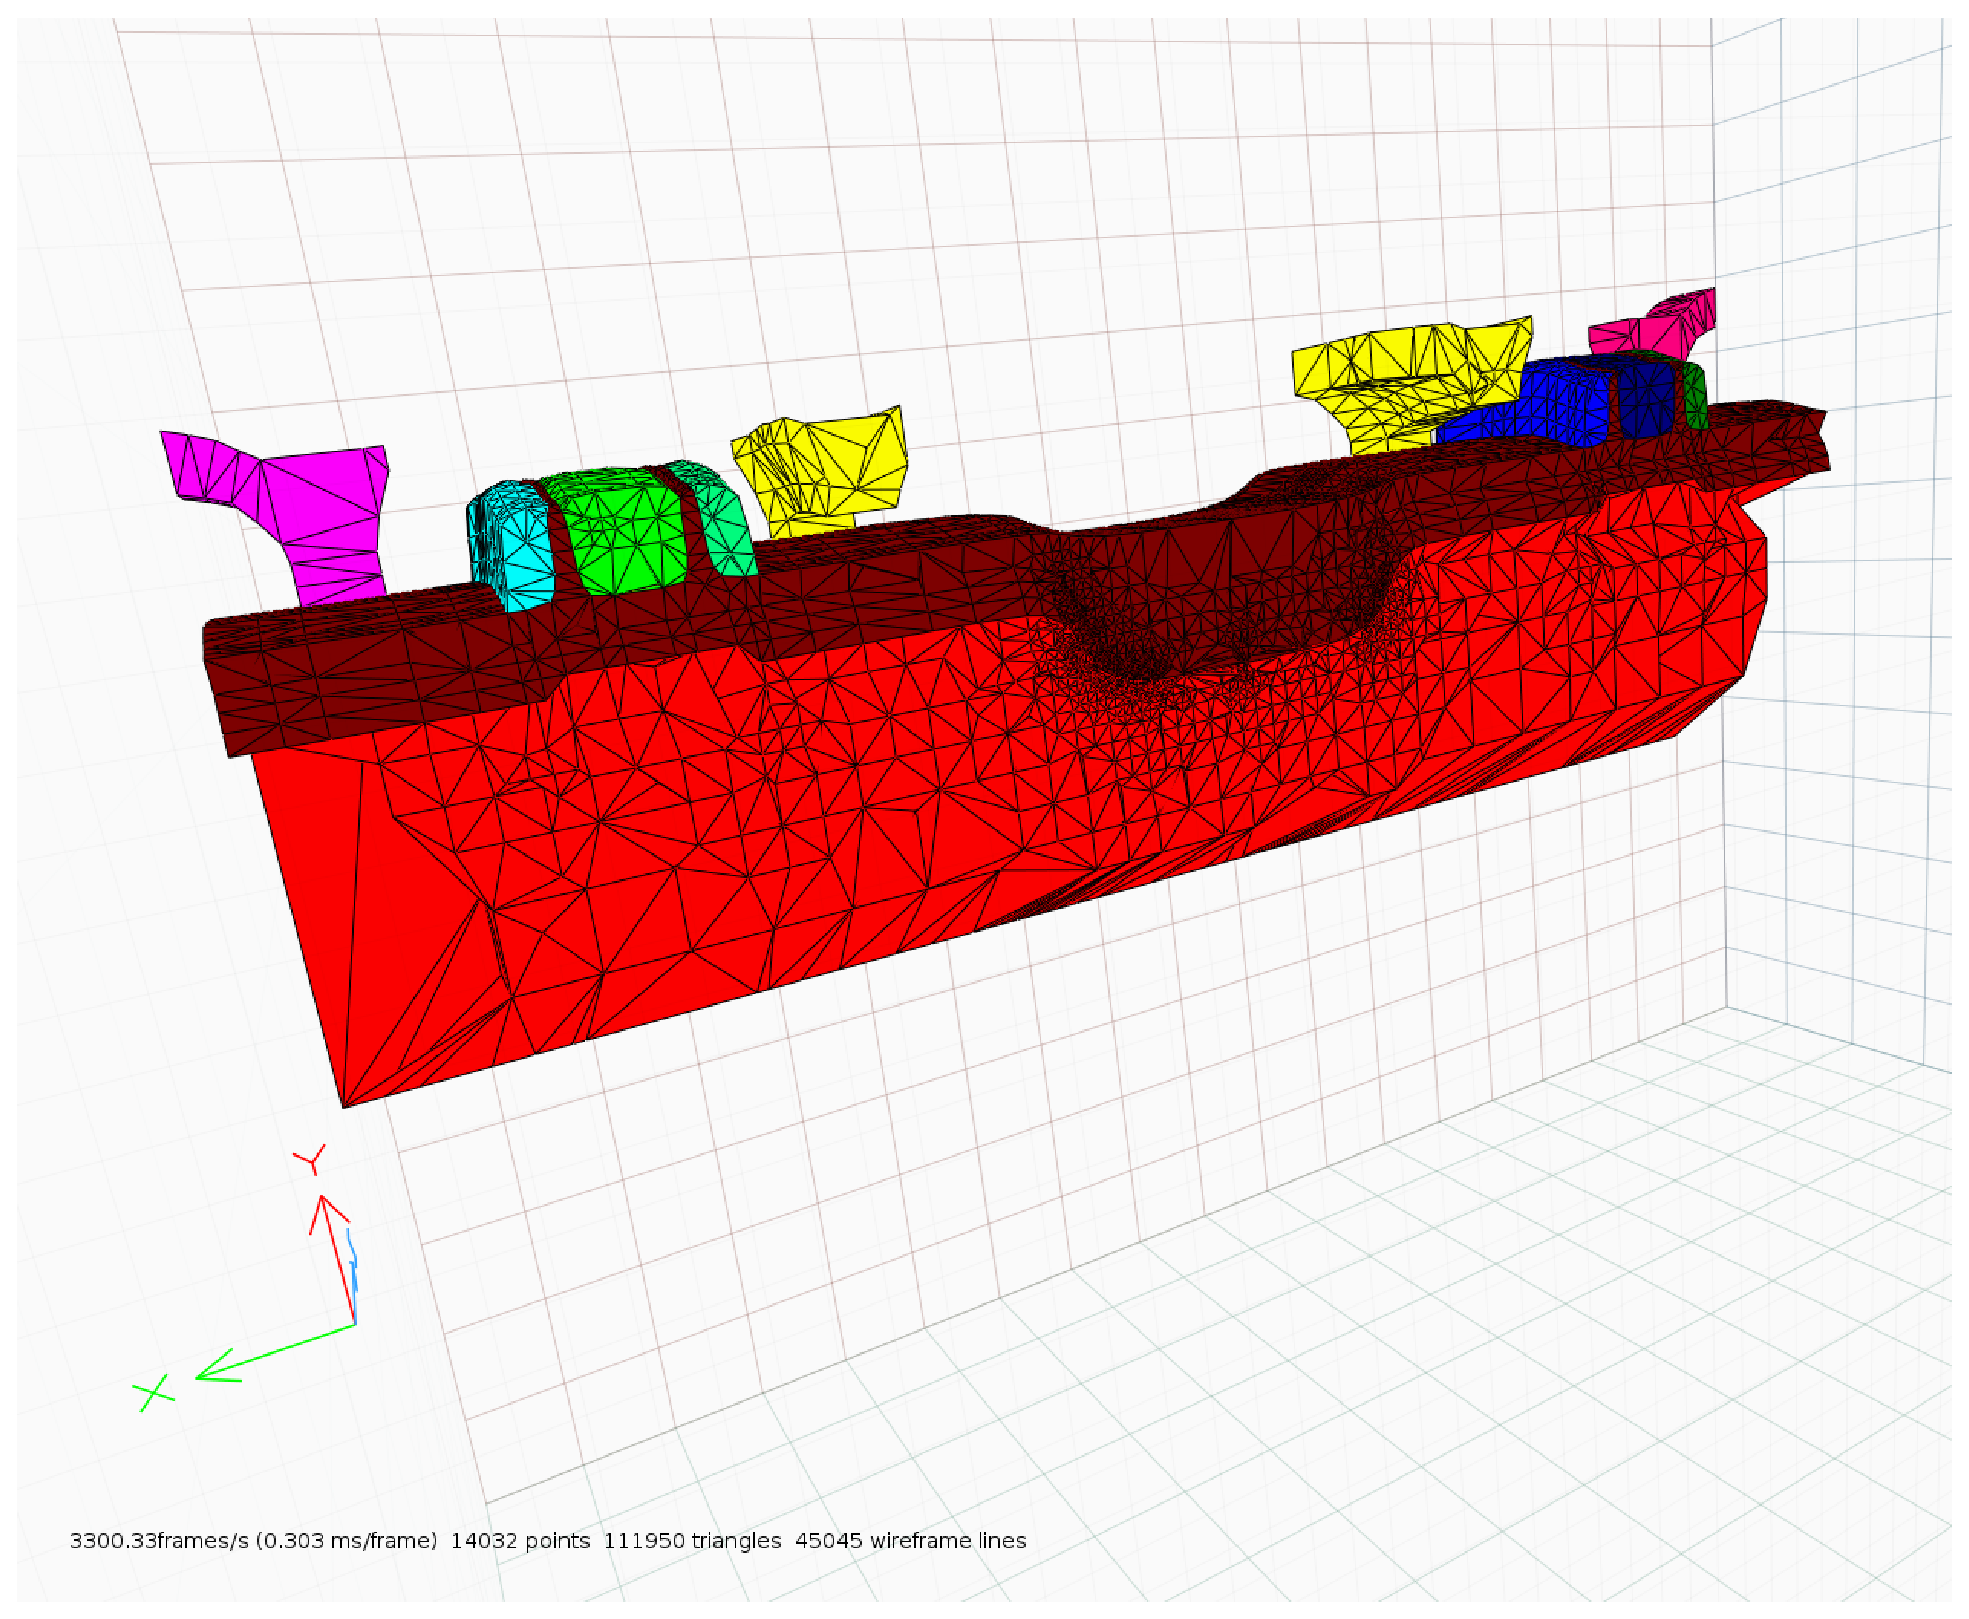
\includegraphics[scale=0.2]{figures/raw/cmos_orig_cut.eps}}
   }
   \subfloat%[\textsc{Adapted Mesh}]
   {
      \fbox{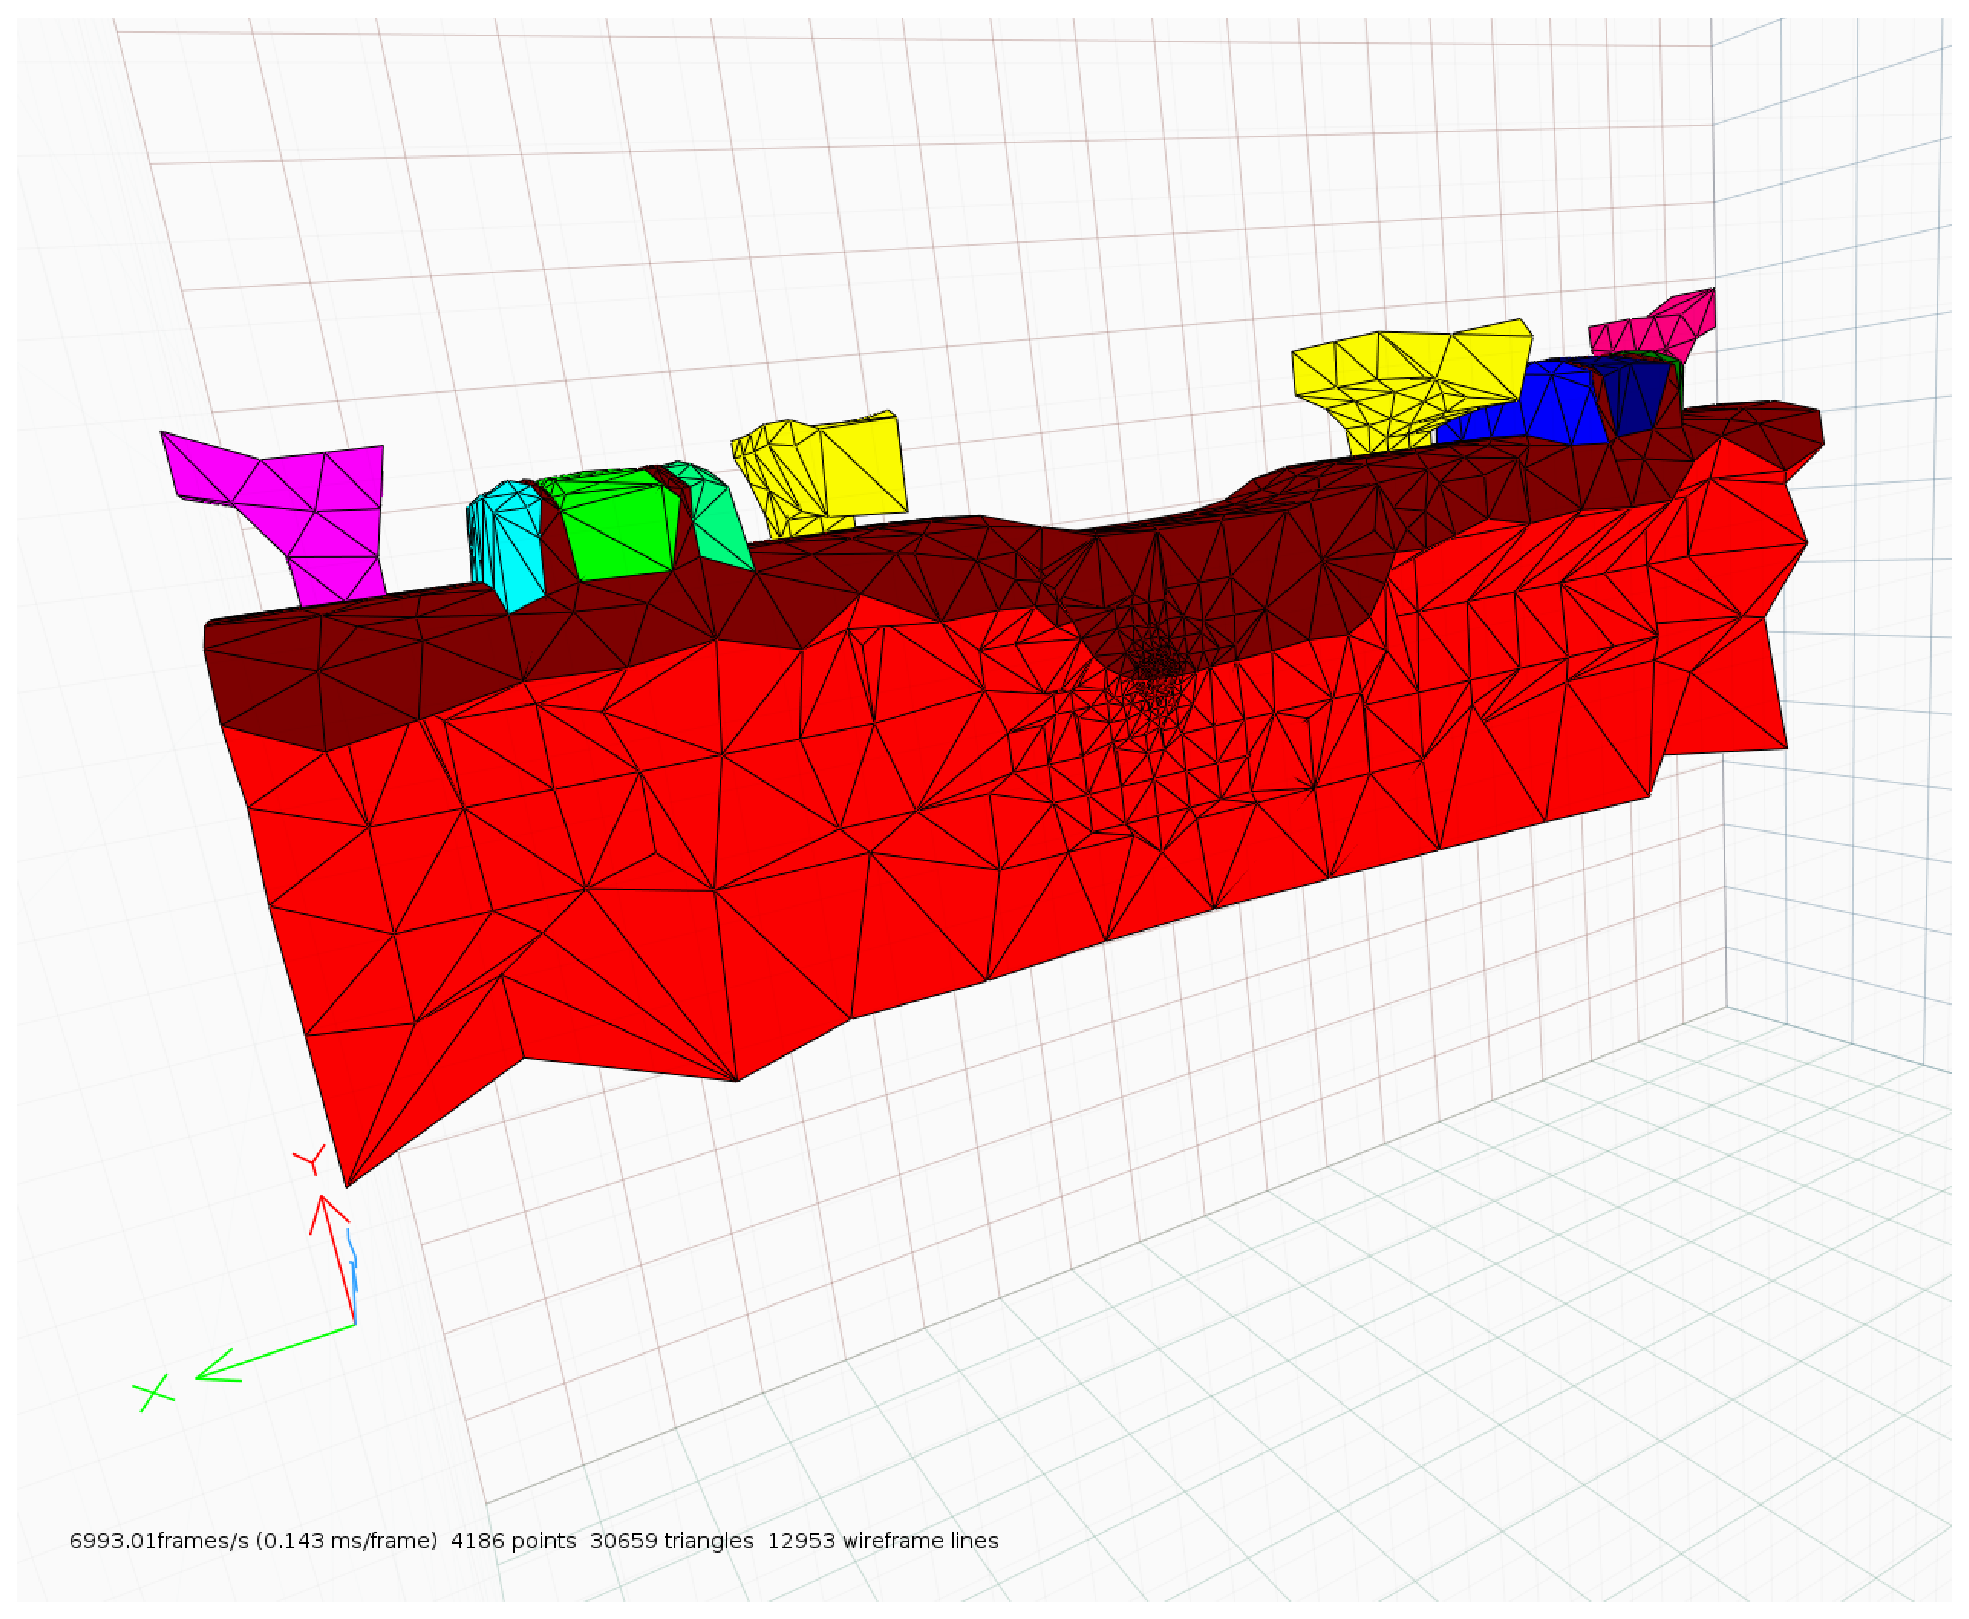
\includegraphics[scale=0.20]{figures/raw/cmos_adapted_cut.eps}}
   }
   \caption{A CMOS structure.\newline 
   \textbf{left:} The initial mesh is shown. \textbf{right:} The adapted mesh is shown.}
\end{figure}


\begin{figure}[!ht]
   \centering

   \subfloat%[\textsc{Initial Mesh}]
   {
      \fbox{
      \begin{tabular}{ccc}
                           & \textbf{original} & \textbf{adapted} \\
      \hline 
      \textbf{vertex size} & 14032             & 4186 \\
      \end{tabular}
      }
   }


   \subfloat%[\textsc{Initial Mesh}]
   {
      \fbox{
      \begin{tabular}{crr}
      cap & 485 & 0.62\% \\
      needle & 3557 & 4.55\% \\
      round & 51745 & 66.16\% \\
      slat & 4363 & 5.58\% \\
      sliver & 4037 & 5.16\% \\
      spade & 1082 & 1.38\% \\
      spindle & 513 & 0.66\% \\
      wedge & 12435 & 15.90\% \\
      \end{tabular}
      }
   }
   \subfloat%[\textsc{Adapted Mesh}]
   {
      \fbox{
      \begin{tabular}{crr}
      cap & 108 & 0.52\% \\
      needle & 393 & 1.88\% \\
      round & 15842 & 75.63\% \\
      slat & 817 & 3.90\% \\
      sliver & 1399 & 6.68\% \\
      spade & 320 & 1.53\% \\
      spindle & 140 & 0.67\% \\
      wedge & 1929 & 9.21\% \\
      \end{tabular}
      }
   }

   \subfloat%[\textsc{Initial Mesh}]
   {
      \fbox{
      \setlength{\unitlength}{1cm}
      \psset{xunit=0.7cm, yunit=0.03017058cm}
      \begin{pspicture}(-1.0,-35.00000000)(10.66666667,130)
      \psaxes[labels=y,Dx=1,Dy=50.](0,0)(8,100)
      \pspolygon[fillcolor=black, fillstyle=solid](-0.08,104.55414013)(0,109.53290870)(0.08,104.55414013)
      \psframe[linewidth=1pt, fillcolor=gray, fillstyle=solid] (0.30000000,0)(0.70000000,0.62)
      \rput[bl](0.35000000,-35.00){\rotateleft{\footnotesize cap}}
      \psframe[linewidth=1pt, fillcolor=gray, fillstyle=solid] (1.30000000,0)(1.70000000,4.55)
      \rput[bl](1.35000000,-35.00){\rotateleft{\footnotesize needle}}
      \psframe[linewidth=1pt, fillcolor=gray, fillstyle=solid] (2.30000000,0)(2.70000000,66.16)
      \rput[bl](2.35000000,-35.00){\rotateleft{\footnotesize round}}
      \psframe[linewidth=1pt, fillcolor=gray, fillstyle=solid] (3.30000000,0)(3.70000000,5.58)
      \rput[bl](3.35000000,-35.00){\rotateleft{\footnotesize slat}}
      \psframe[linewidth=1pt, fillcolor=gray, fillstyle=solid] (4.30000000,0)(4.70000000,5.16)
      \rput[bl](4.35000000,-35.00){\rotateleft{\footnotesize sliver}}
      \psframe[linewidth=1pt, fillcolor=gray, fillstyle=solid] (5.30000000,0)(5.70000000,1.38)
      \rput[bl](5.35000000,-35.00){\rotateleft{\footnotesize spade}}
      \psframe[linewidth=1pt, fillcolor=gray, fillstyle=solid] (6.30000000,0)(6.70000000,0.66)
      \rput[bl](6.35000000,-35.00){\rotateleft{\footnotesize spindle}}
      \psframe[linewidth=1pt, fillcolor=gray, fillstyle=solid] (7.30000000,0)(7.70000000,15.90)
      \rput[bl](7.35000000,-35.00){\rotateleft{\footnotesize wedge}}
      \end{pspicture}
      }
   }
   \subfloat%[\textsc{Adapted Mesh}]
   {
      \fbox{
      \setlength{\unitlength}{1cm}
      \psset{xunit=0.7cm, yunit=0.03017058cm}
      \begin{pspicture}(-1.0,-35.00000000)(10.66666667,130)
      \psaxes[labels=y,Dx=1,Dy=50.](0,0)(8,100)
      \pspolygon[fillcolor=black, fillstyle=solid](-0.08,104.55414013)(0,109.53290870)(0.08,104.55414013)
      \psframe[linewidth=1pt, fillcolor=gray, fillstyle=solid] (0.30000000,0)(0.70000000,0.52)
      \rput[bl](0.35000000,-35.00){\rotateleft{\footnotesize cap}}
      \psframe[linewidth=1pt, fillcolor=gray, fillstyle=solid] (1.30000000,0)(1.70000000,1.88)
      \rput[bl](1.35000000,-35.00){\rotateleft{\footnotesize needle}}
      \psframe[linewidth=1pt, fillcolor=gray, fillstyle=solid] (2.30000000,0)(2.70000000,75.63)
      \rput[bl](2.35000000,-35.00){\rotateleft{\footnotesize round}}
      \psframe[linewidth=1pt, fillcolor=gray, fillstyle=solid] (3.30000000,0)(3.70000000,3.90)
      \rput[bl](3.35000000,-35.00){\rotateleft{\footnotesize slat}}
      \psframe[linewidth=1pt, fillcolor=gray, fillstyle=solid] (4.30000000,0)(4.70000000,6.68)
      \rput[bl](4.35000000,-35.00){\rotateleft{\footnotesize sliver}}
      \psframe[linewidth=1pt, fillcolor=gray, fillstyle=solid] (5.30000000,0)(5.70000000,1.53)
      \rput[bl](5.35000000,-35.00){\rotateleft{\footnotesize spade}}
      \psframe[linewidth=1pt, fillcolor=gray, fillstyle=solid] (6.30000000,0)(6.70000000,0.67)
      \rput[bl](6.35000000,-35.00){\rotateleft{\footnotesize spindle}}
      \psframe[linewidth=1pt, fillcolor=gray, fillstyle=solid] (7.30000000,0)(7.70000000,9.21)
      \rput[bl](7.35000000,-35.00){\rotateleft{\footnotesize wedge}}
      \end{pspicture}
      }
   }
   \caption{A mesh quality analysis of the original and the adapted CMOS structure meshes. 
   The analysis of the initial mesh and the adapted mesh is depicted, on the \textbf{left}
   \textbf{right}, respectively. Apparently, the mesh adaption process 
   introduces a bit more \texttt{slivers}, on the other hand, a considerable amount 
   of \texttt{rounds} is introduced too. This result is quite good, as the significant 
   reduction of the vertex size has to be taken into account. 
   }
\end{figure}




\clearpage

\subsection{Etched Hole with Cylindrical Mask}

In the following, different views of the original and the adapted 
volume mesh are presented. Additionally, a comparison of the mesh quality 
is depicted.

\begin{figure}[!ht]
   \centering
   \subfloat%[\textsc{Initial Mesh}]
   {
      \fbox{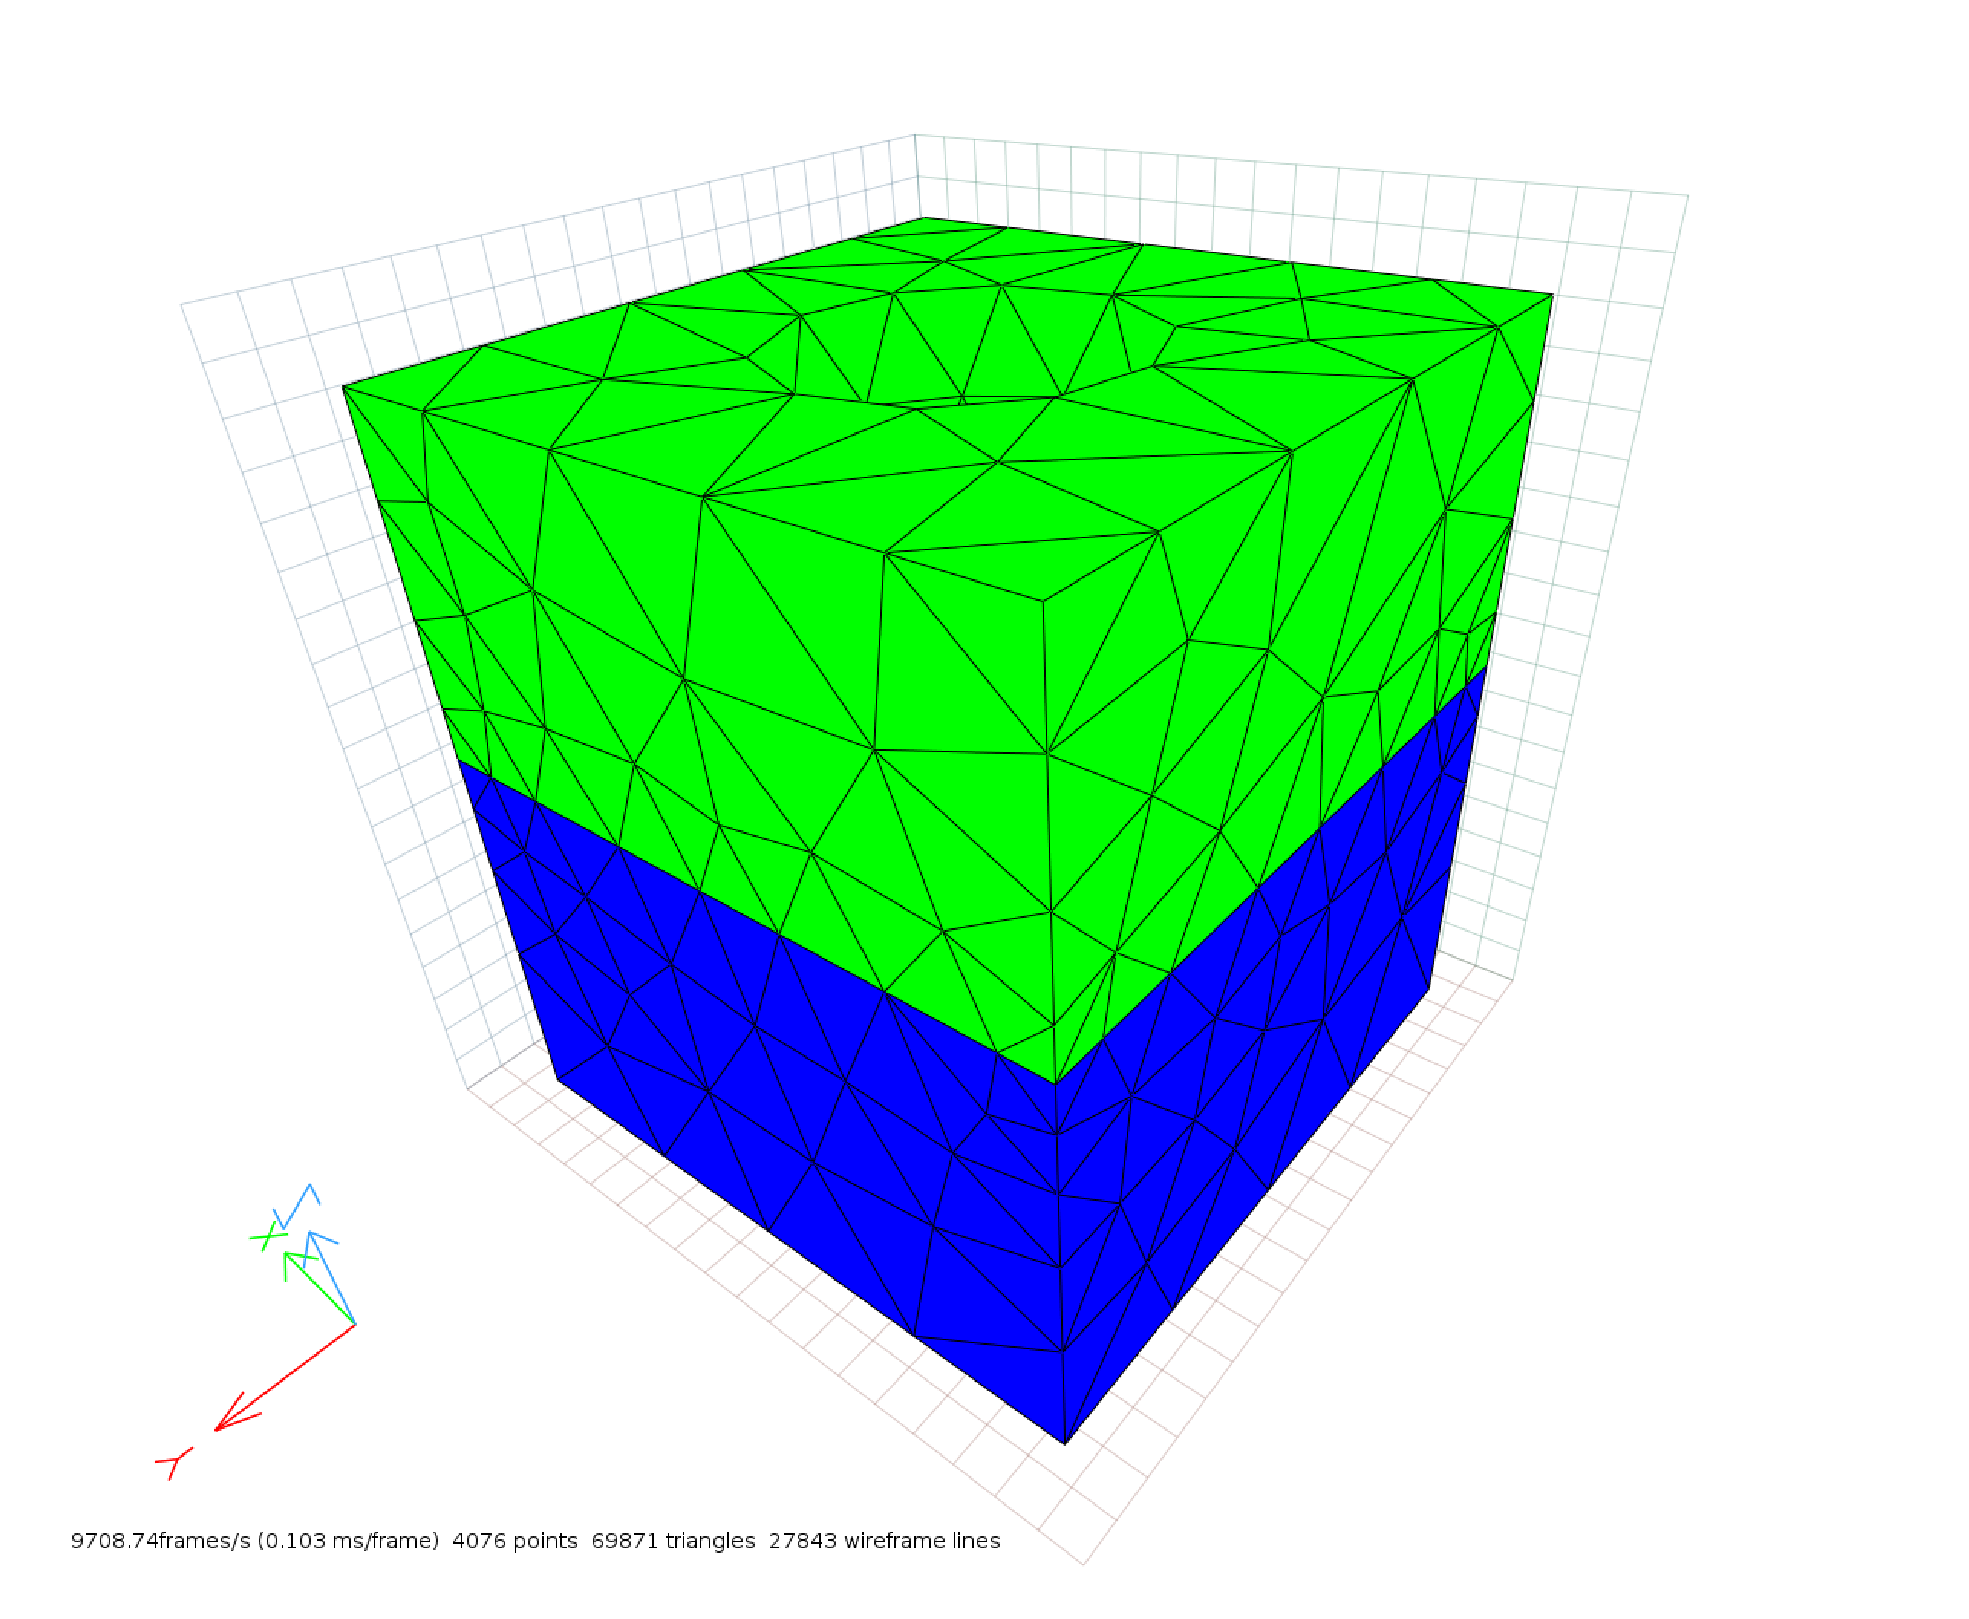
\includegraphics[scale=0.2]{figures/raw/cyl_mask_etched_flux_orig_total.eps}}
   }
   \subfloat%[\textsc{Adapted Mesh}]
   {
      \fbox{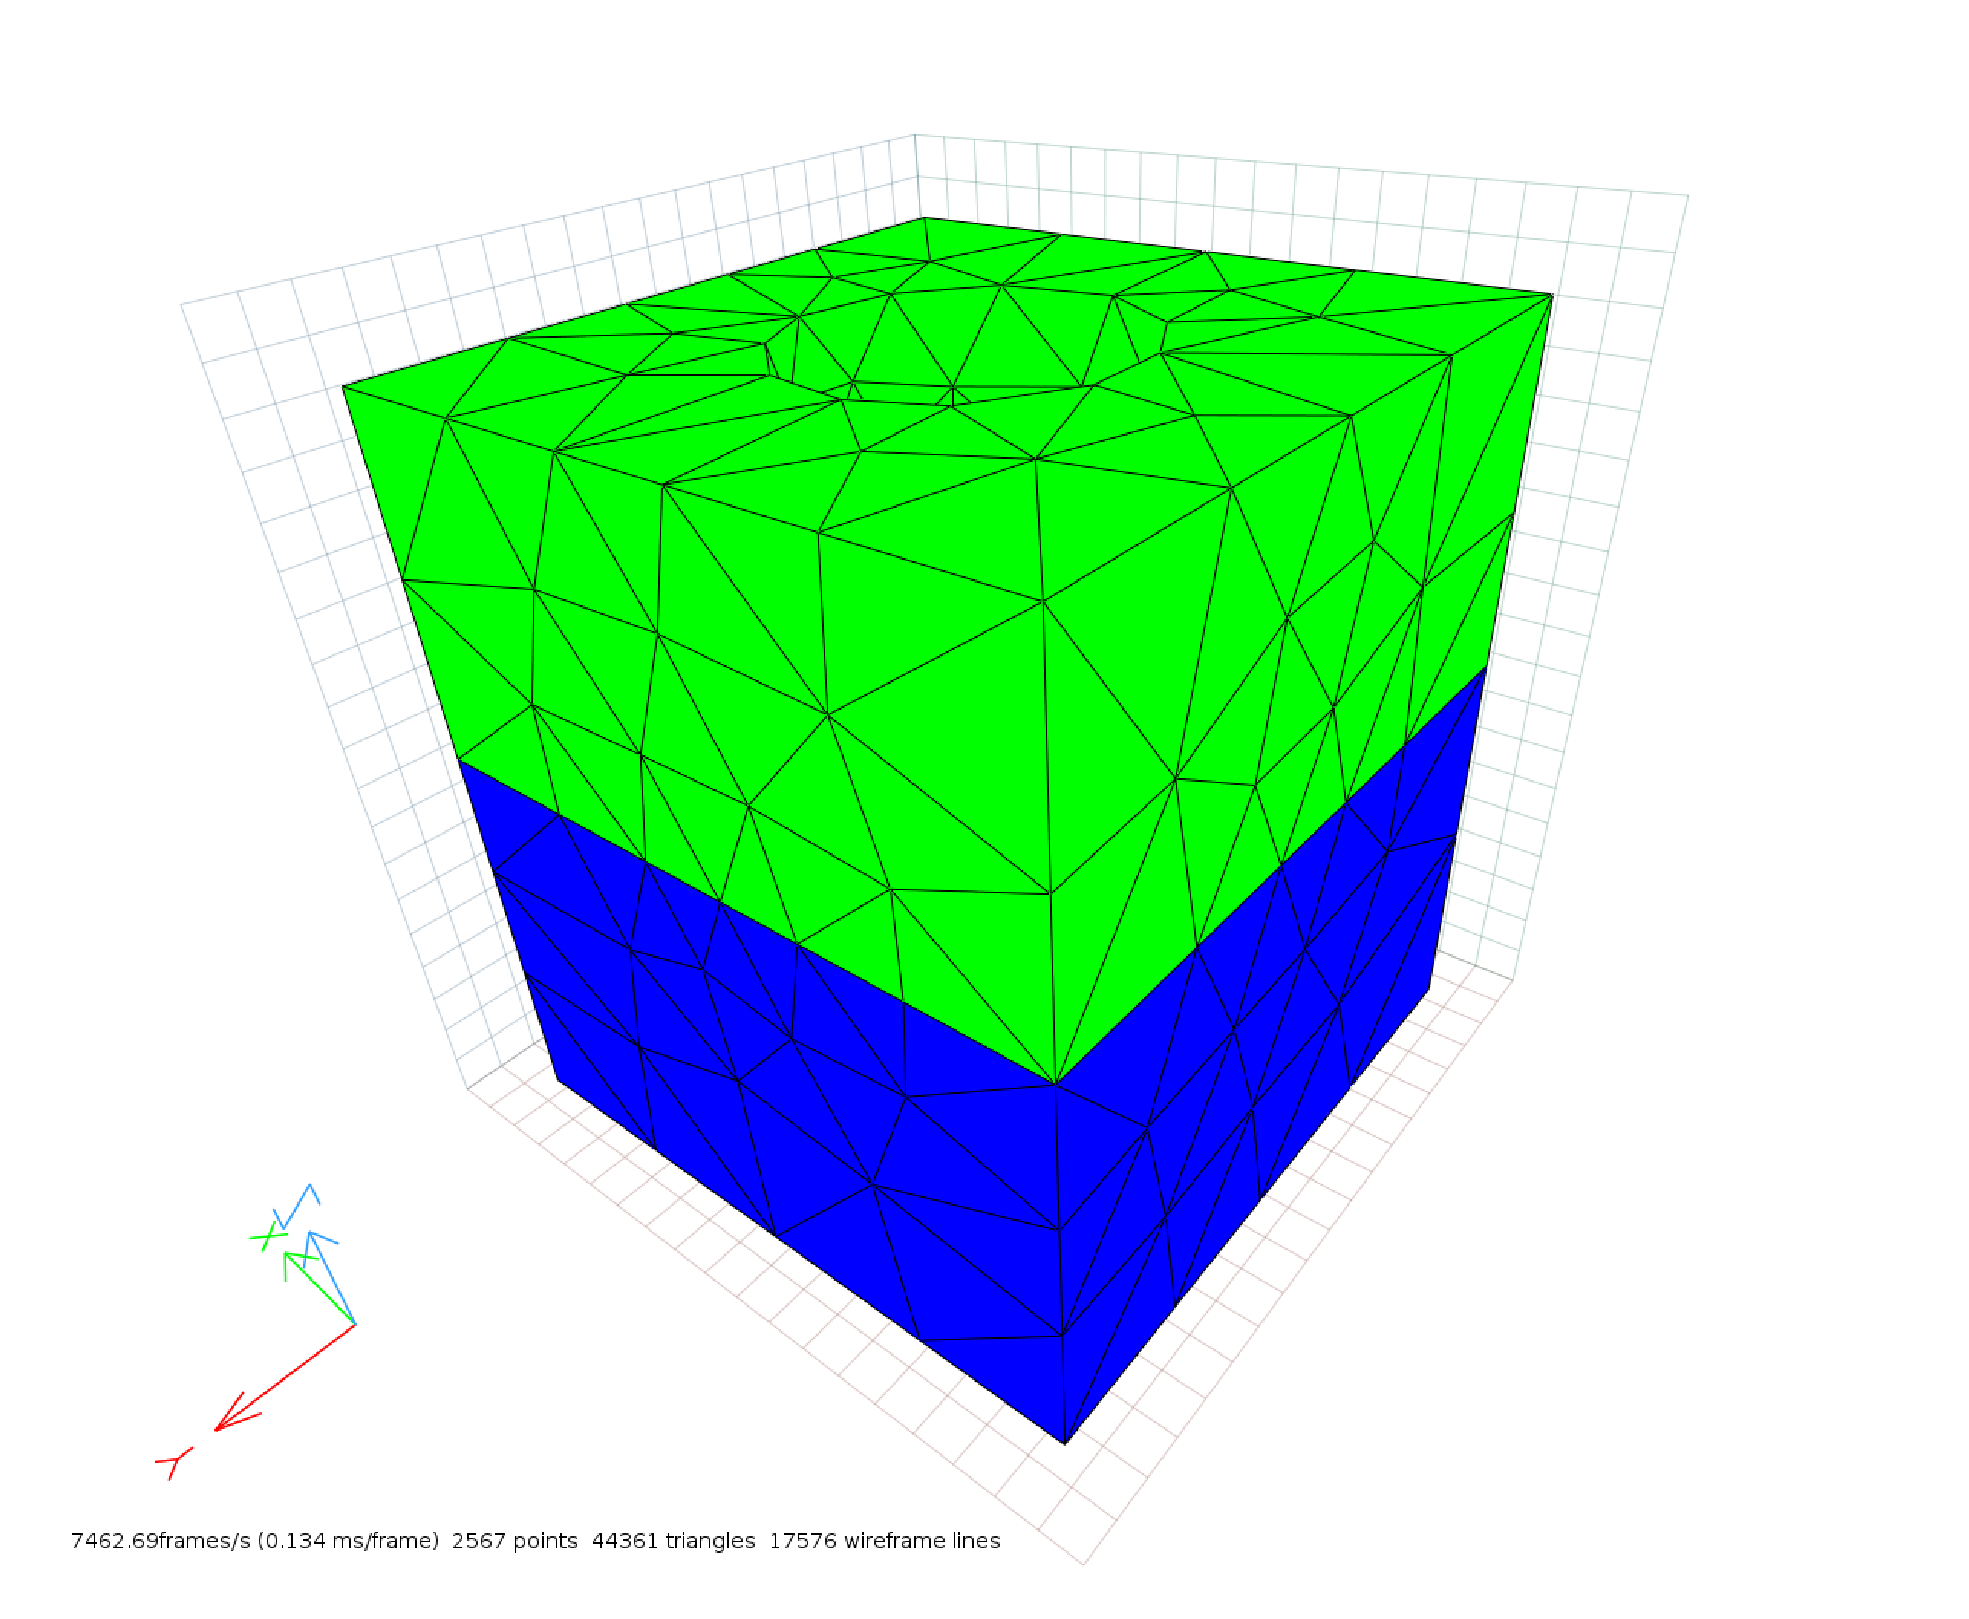
\includegraphics[scale=0.20]{figures/raw/cyl_mask_etched_flux_adapted_total.eps}}
   }

   \subfloat%[\textsc{Initial Mesh}]
   {
      \fbox{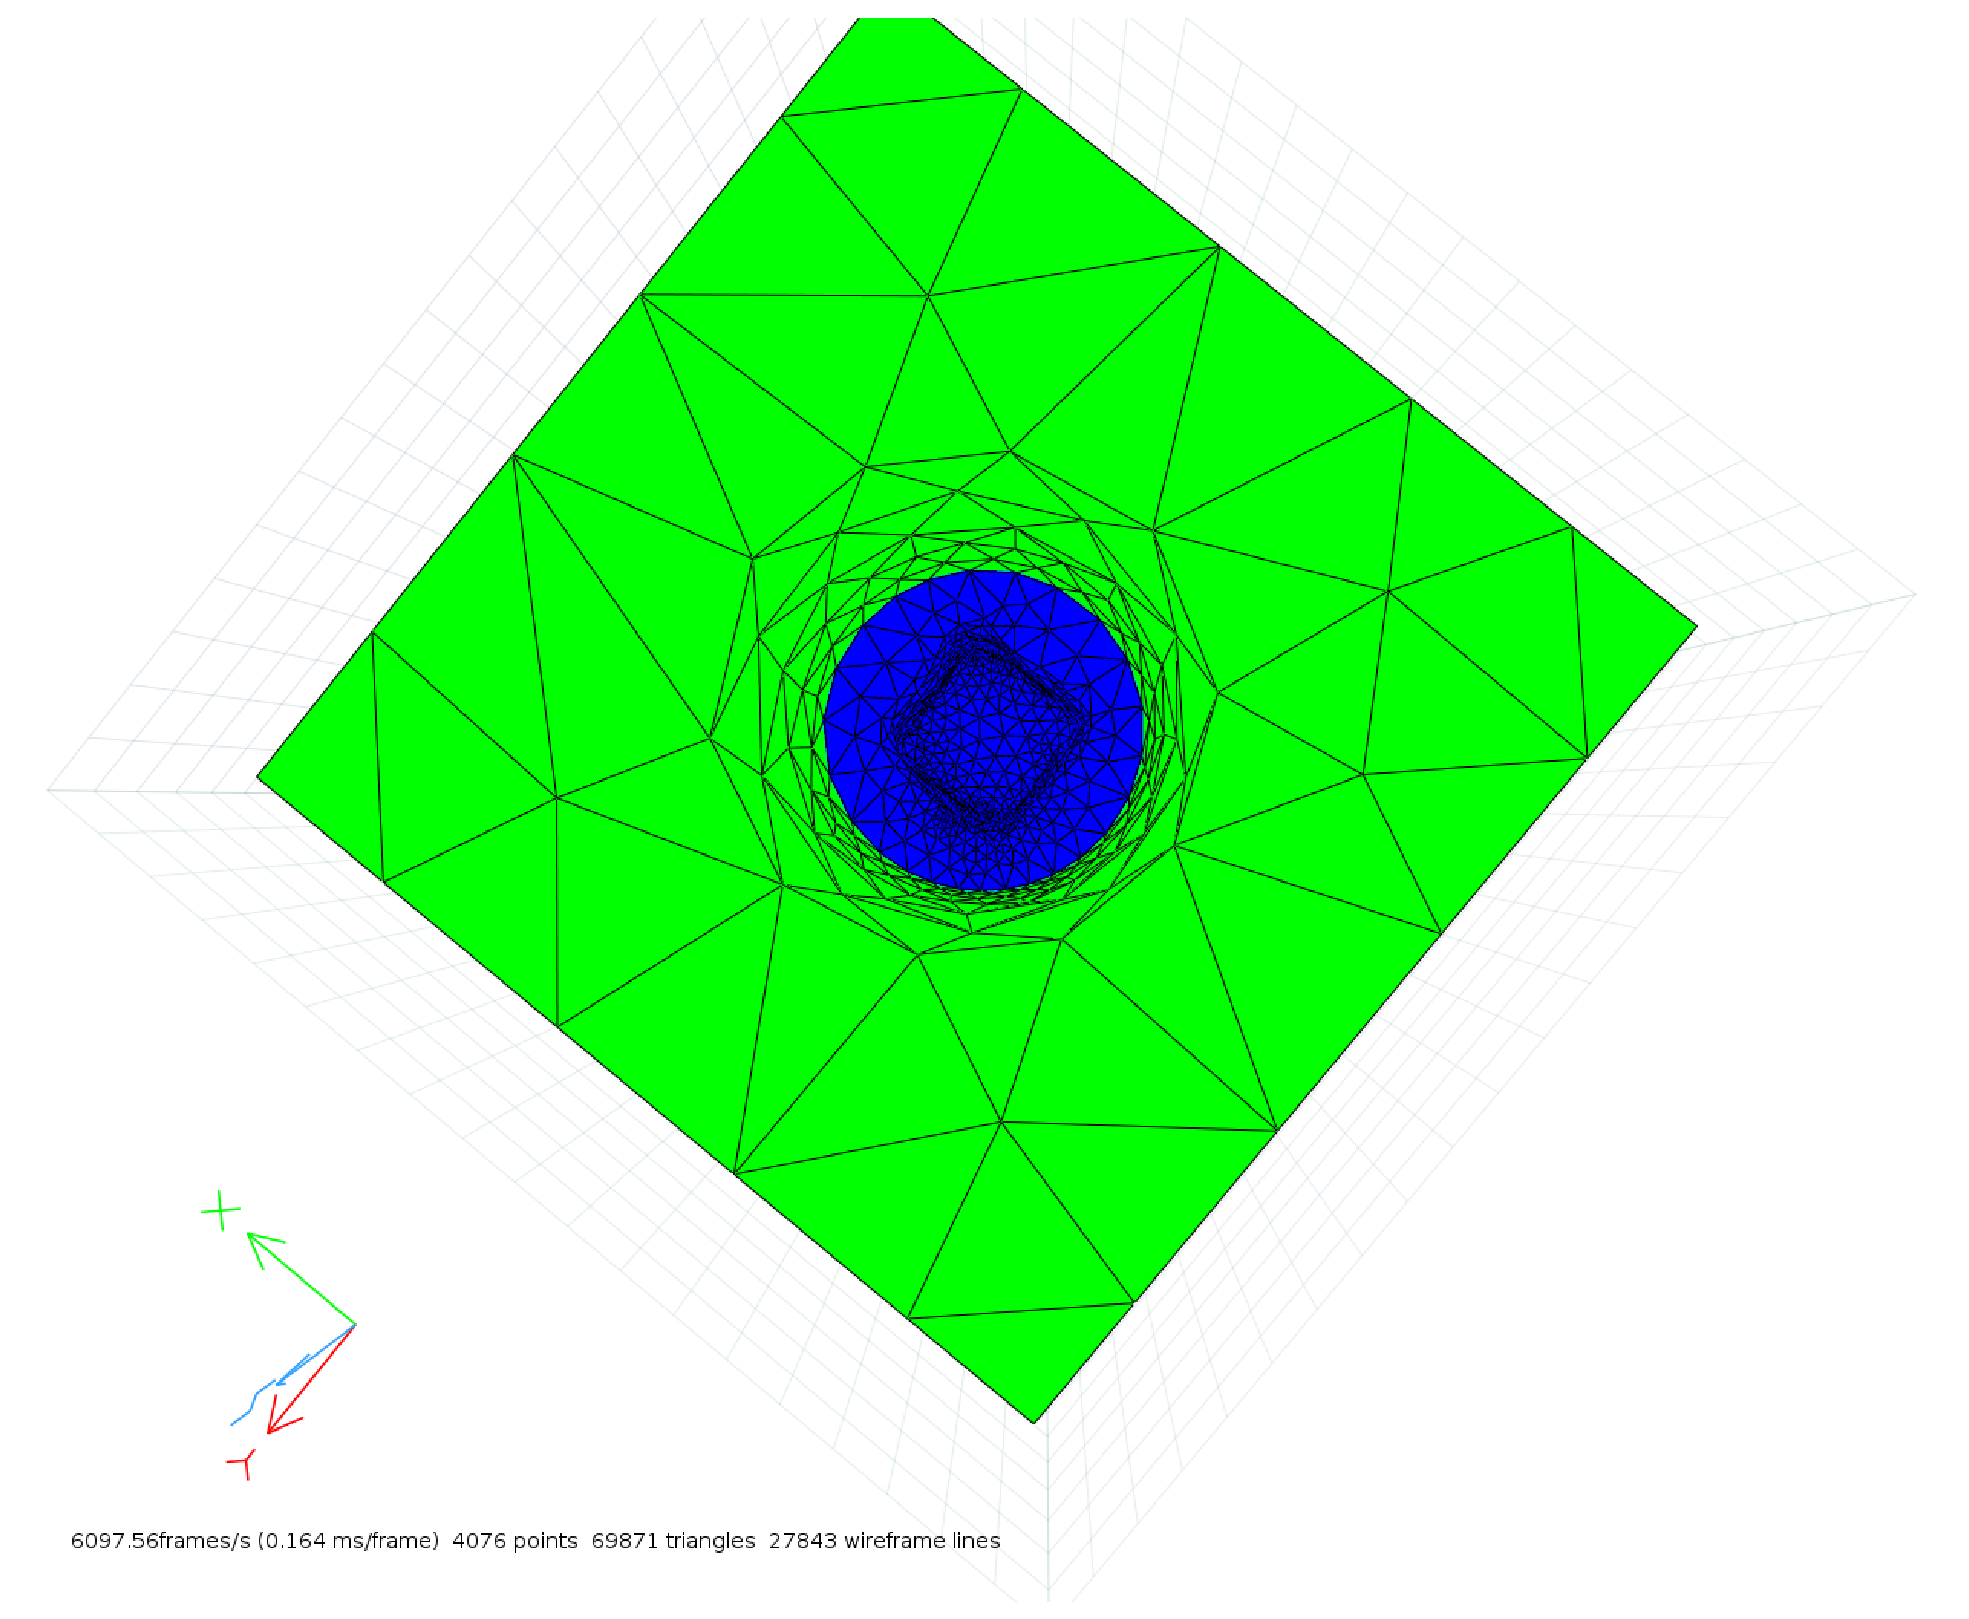
\includegraphics[scale=0.2]{figures/raw/cyl_mask_etched_flux_orig_top.eps}}
   }
   \subfloat%[\textsc{Adapted Mesh}]
   {
      \fbox{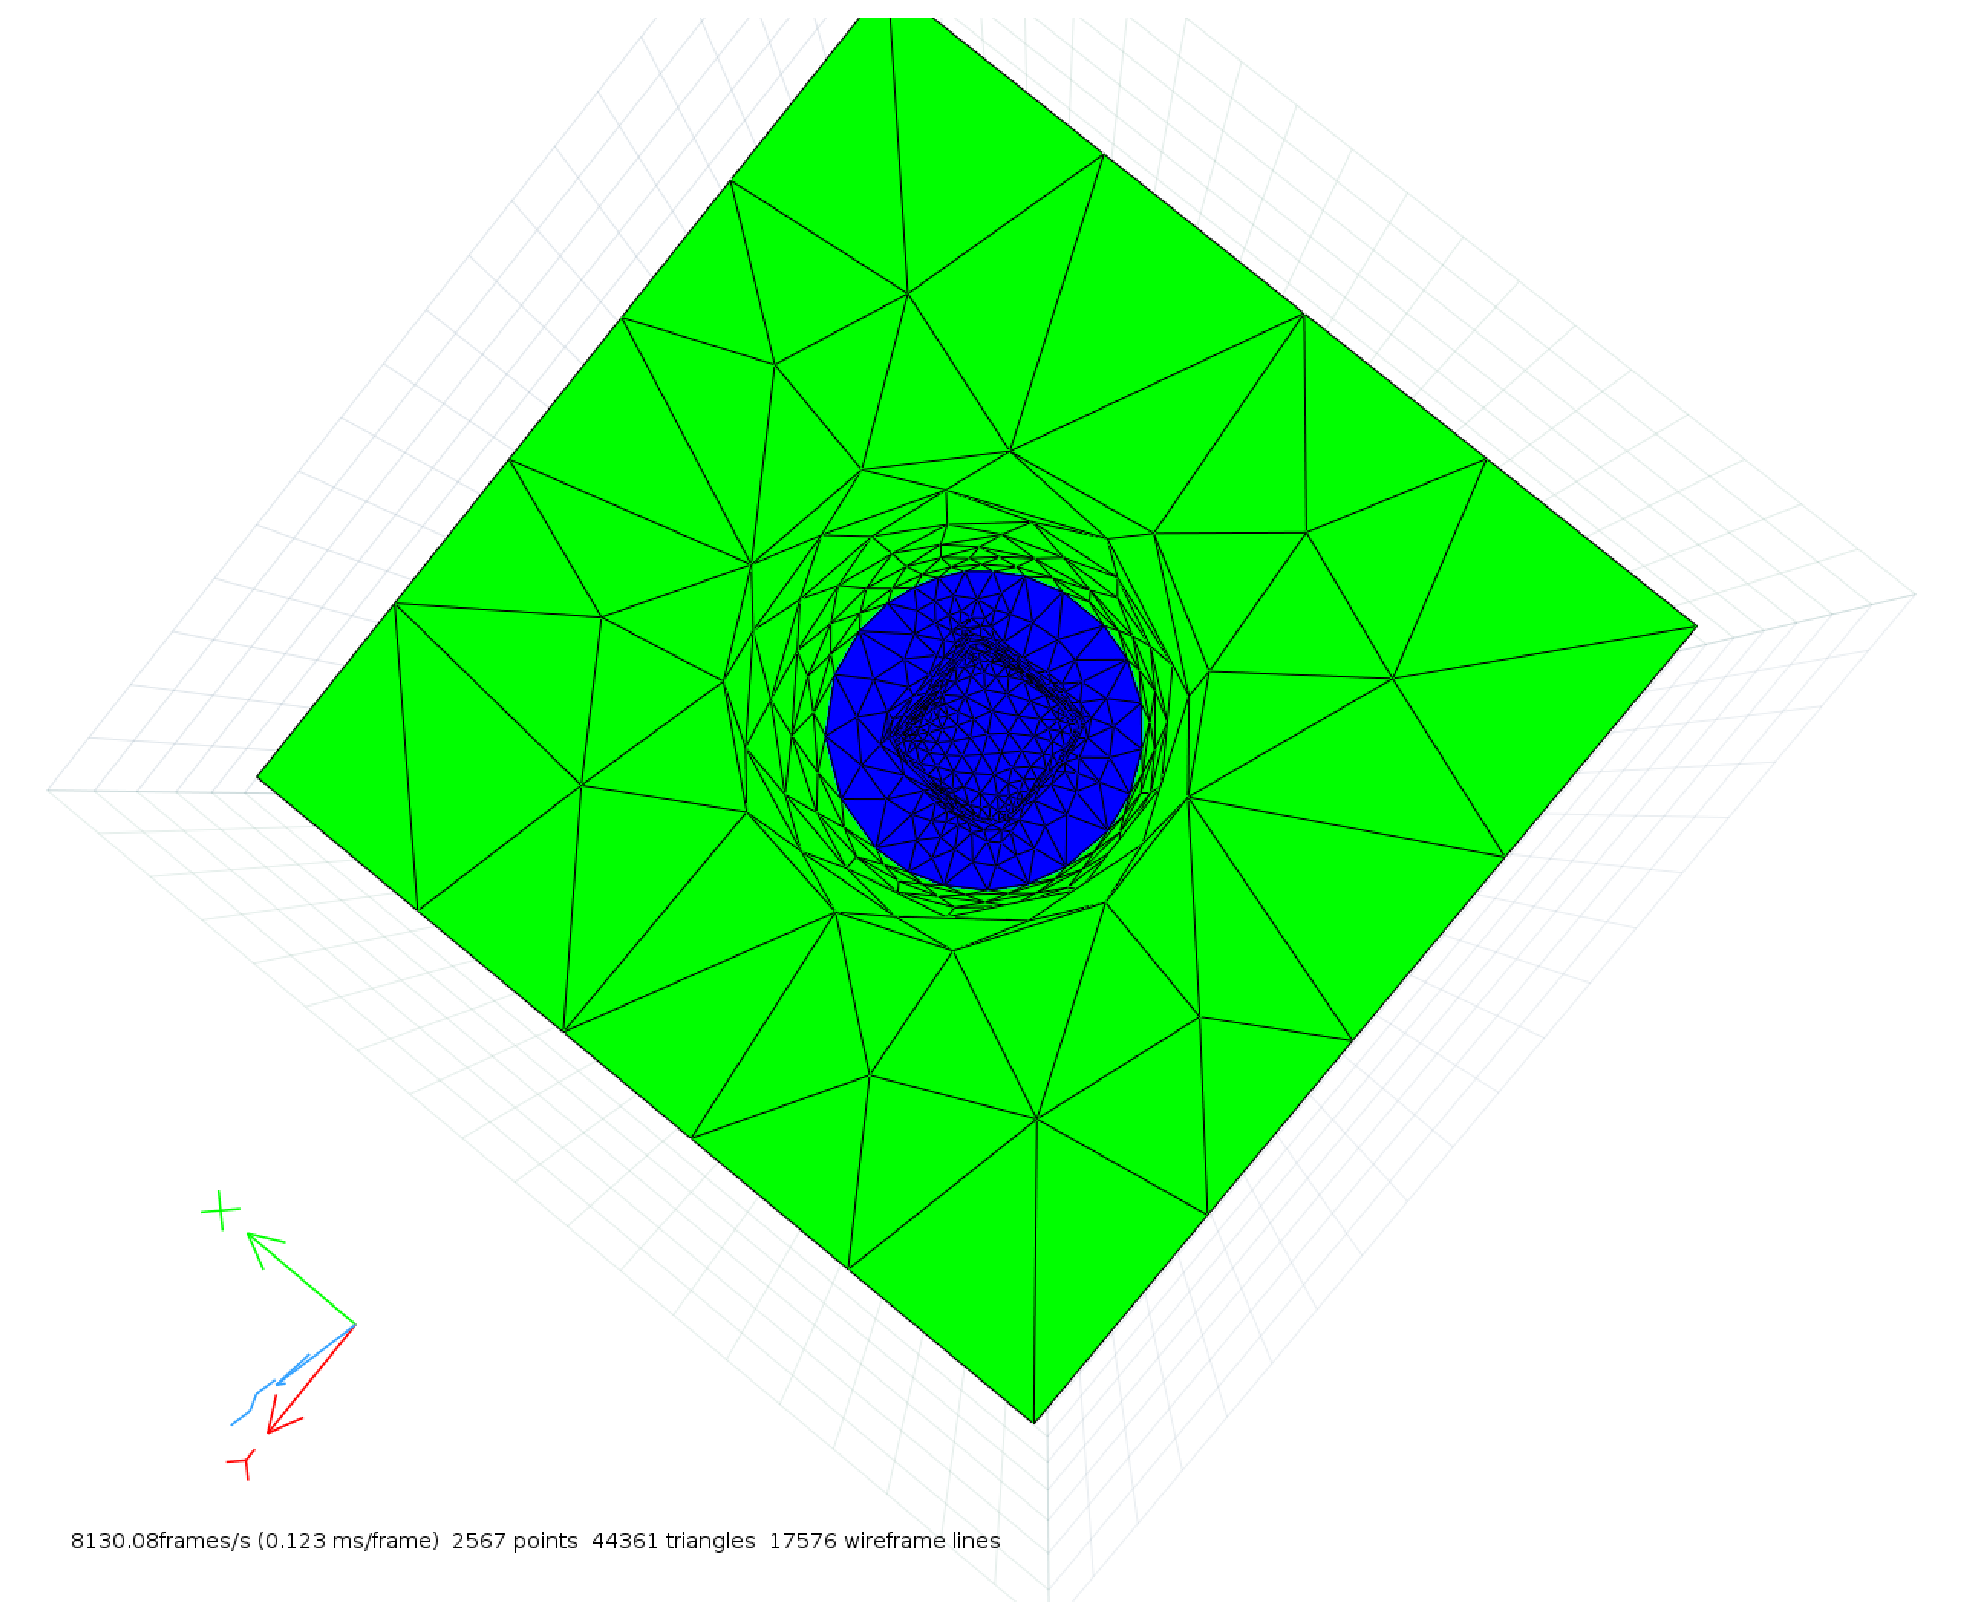
\includegraphics[scale=0.20]{figures/raw/cyl_mask_etched_flux_adapted_top.eps}}
   }
   \caption{Etched hole with cylindrical mask.\newline 
   \textbf{left:} The initial mesh is shown. \textbf{right:} The adapted mesh is shown.}
\end{figure}

\begin{figure}[!ht]
   \centering
   \subfloat%[\textsc{Initial Mesh}]
   {
      \fbox{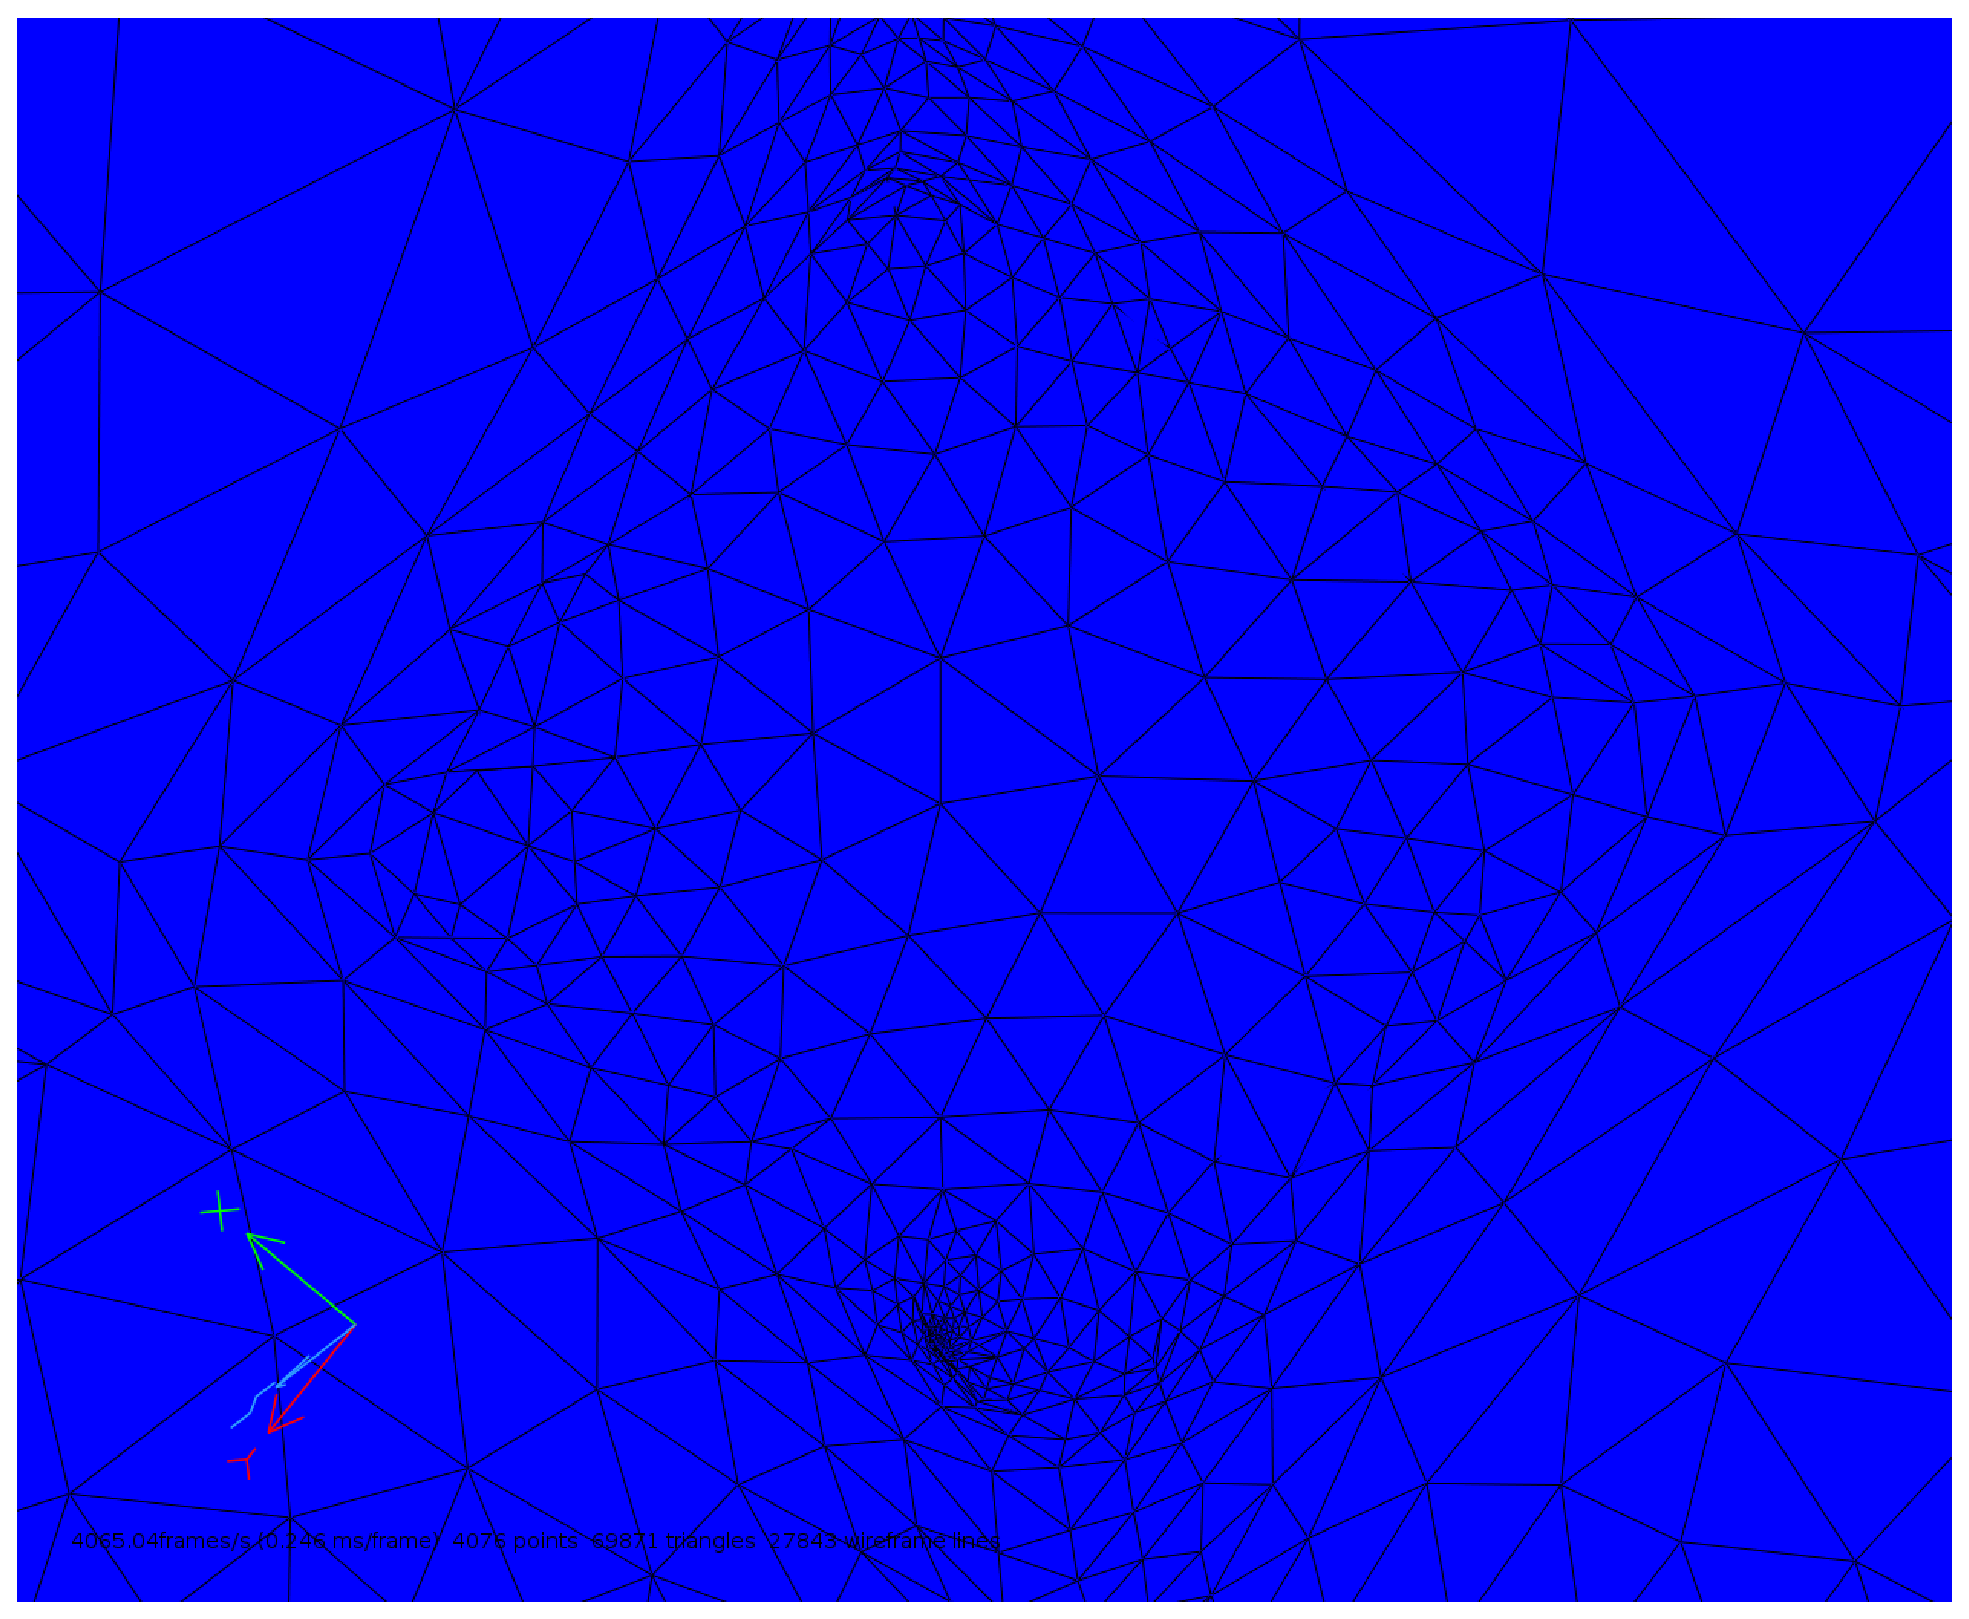
\includegraphics[scale=0.2]{figures/raw/cyl_mask_etched_flux_orig_close.eps}}
   }
   \subfloat%[\textsc{Adapted Mesh}]
   {
      \fbox{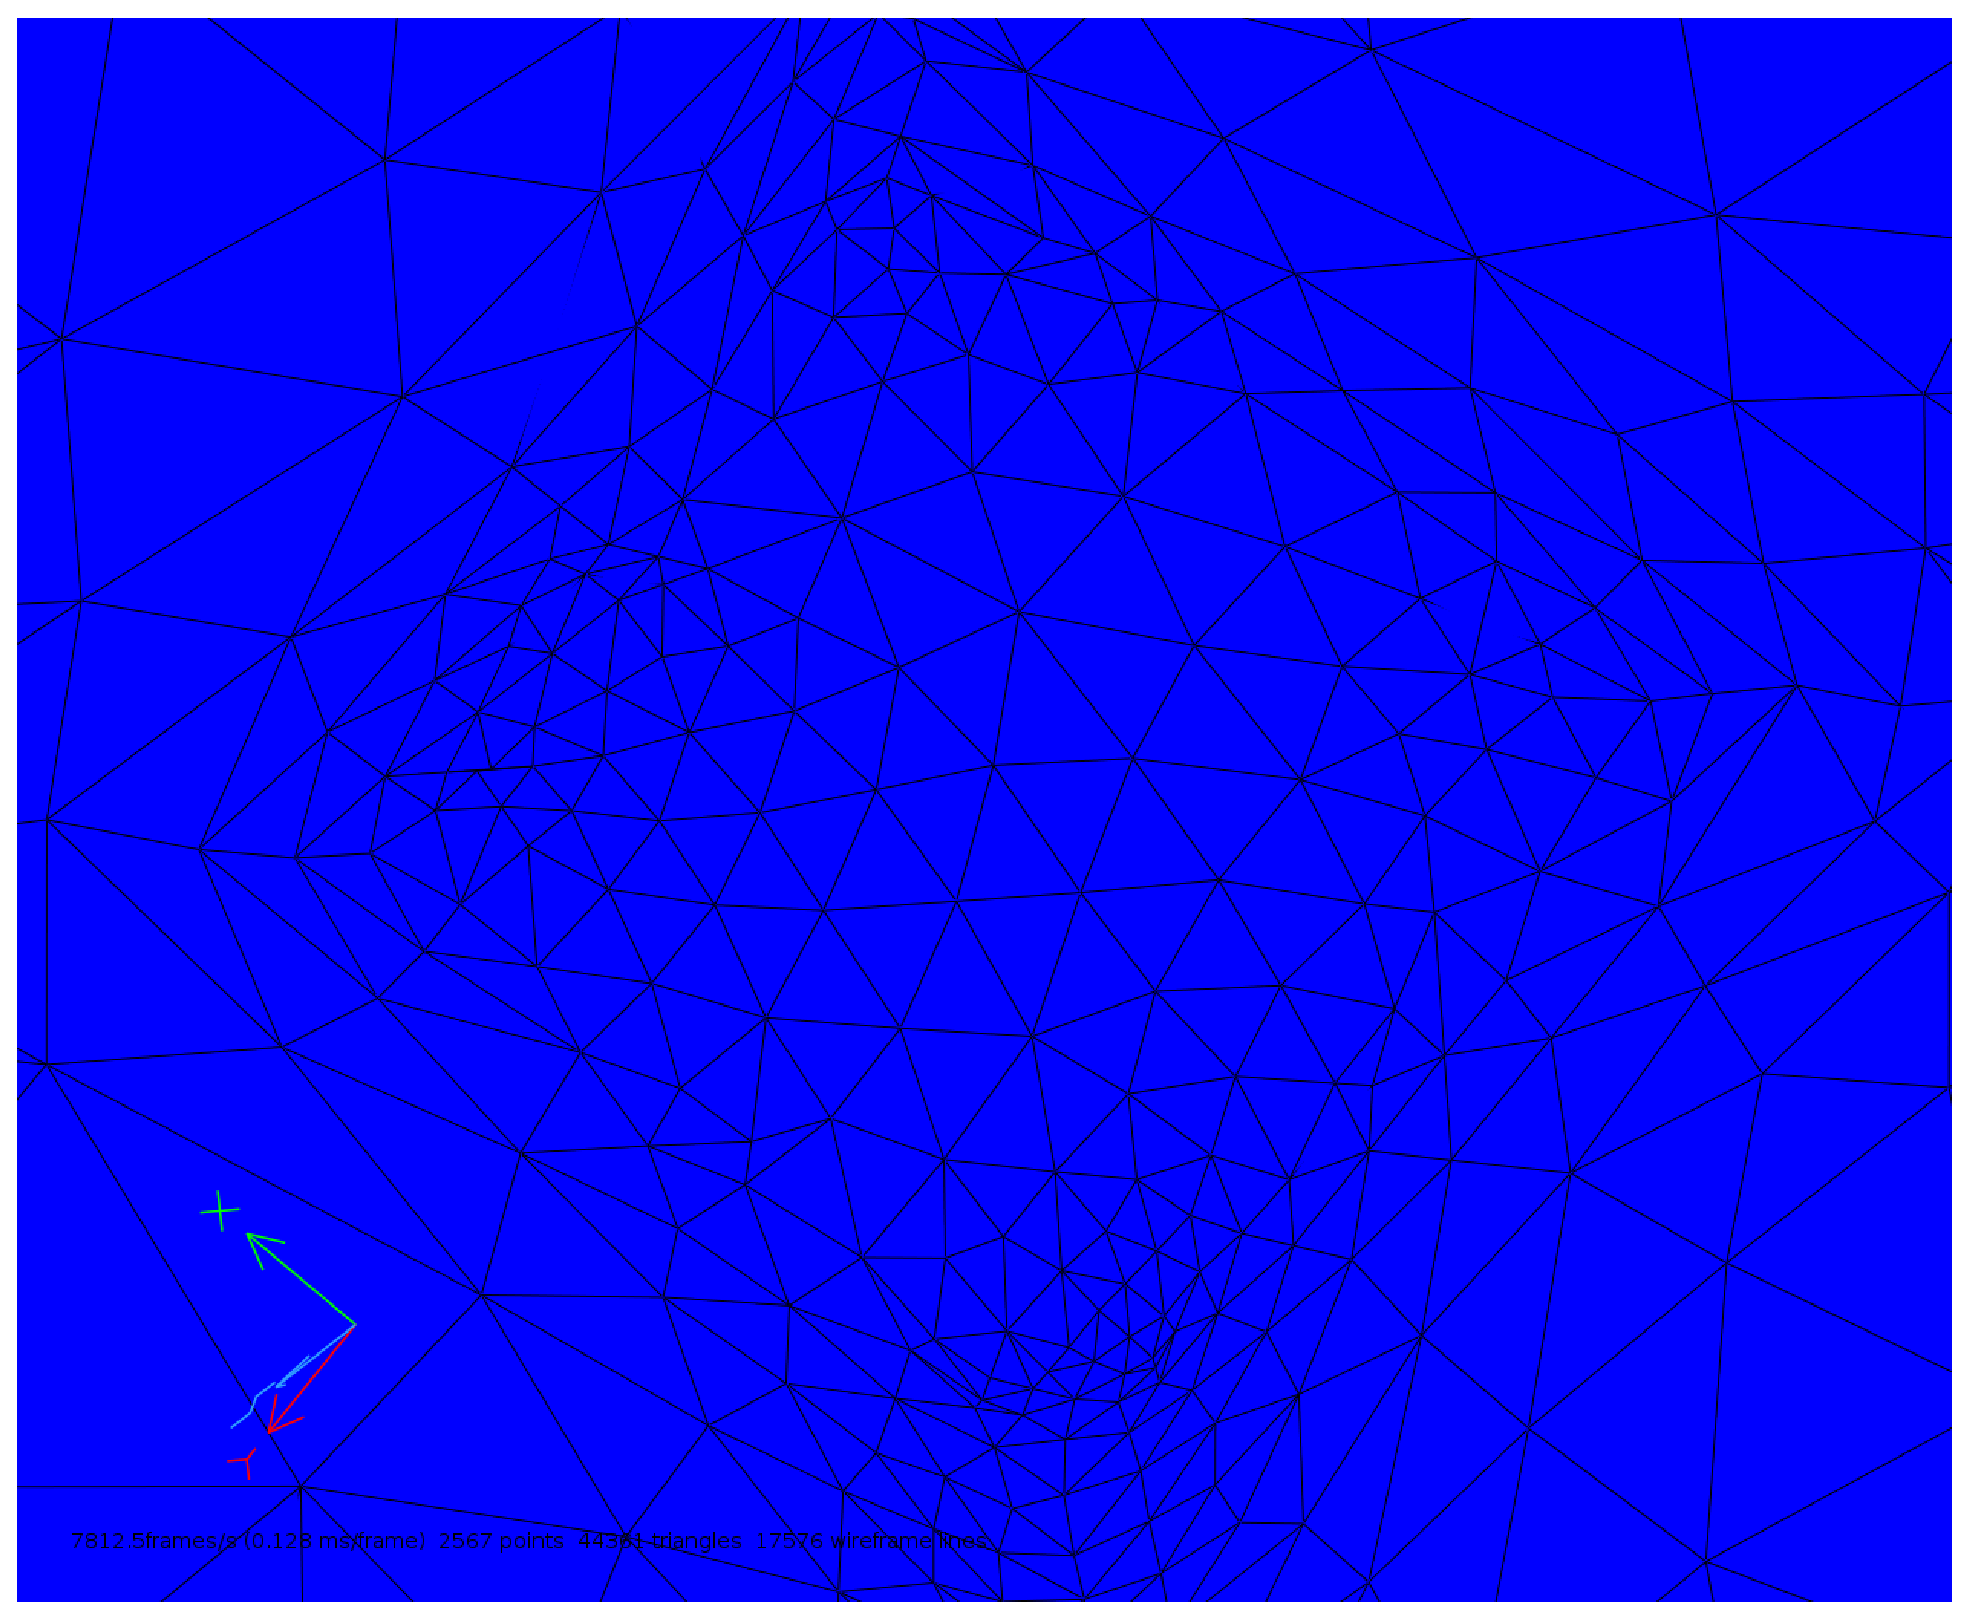
\includegraphics[scale=0.20]{figures/raw/cyl_mask_etched_flux_adapted_close.eps}}
   }

   \subfloat%[\textsc{Initial Mesh}]
   {
      \fbox{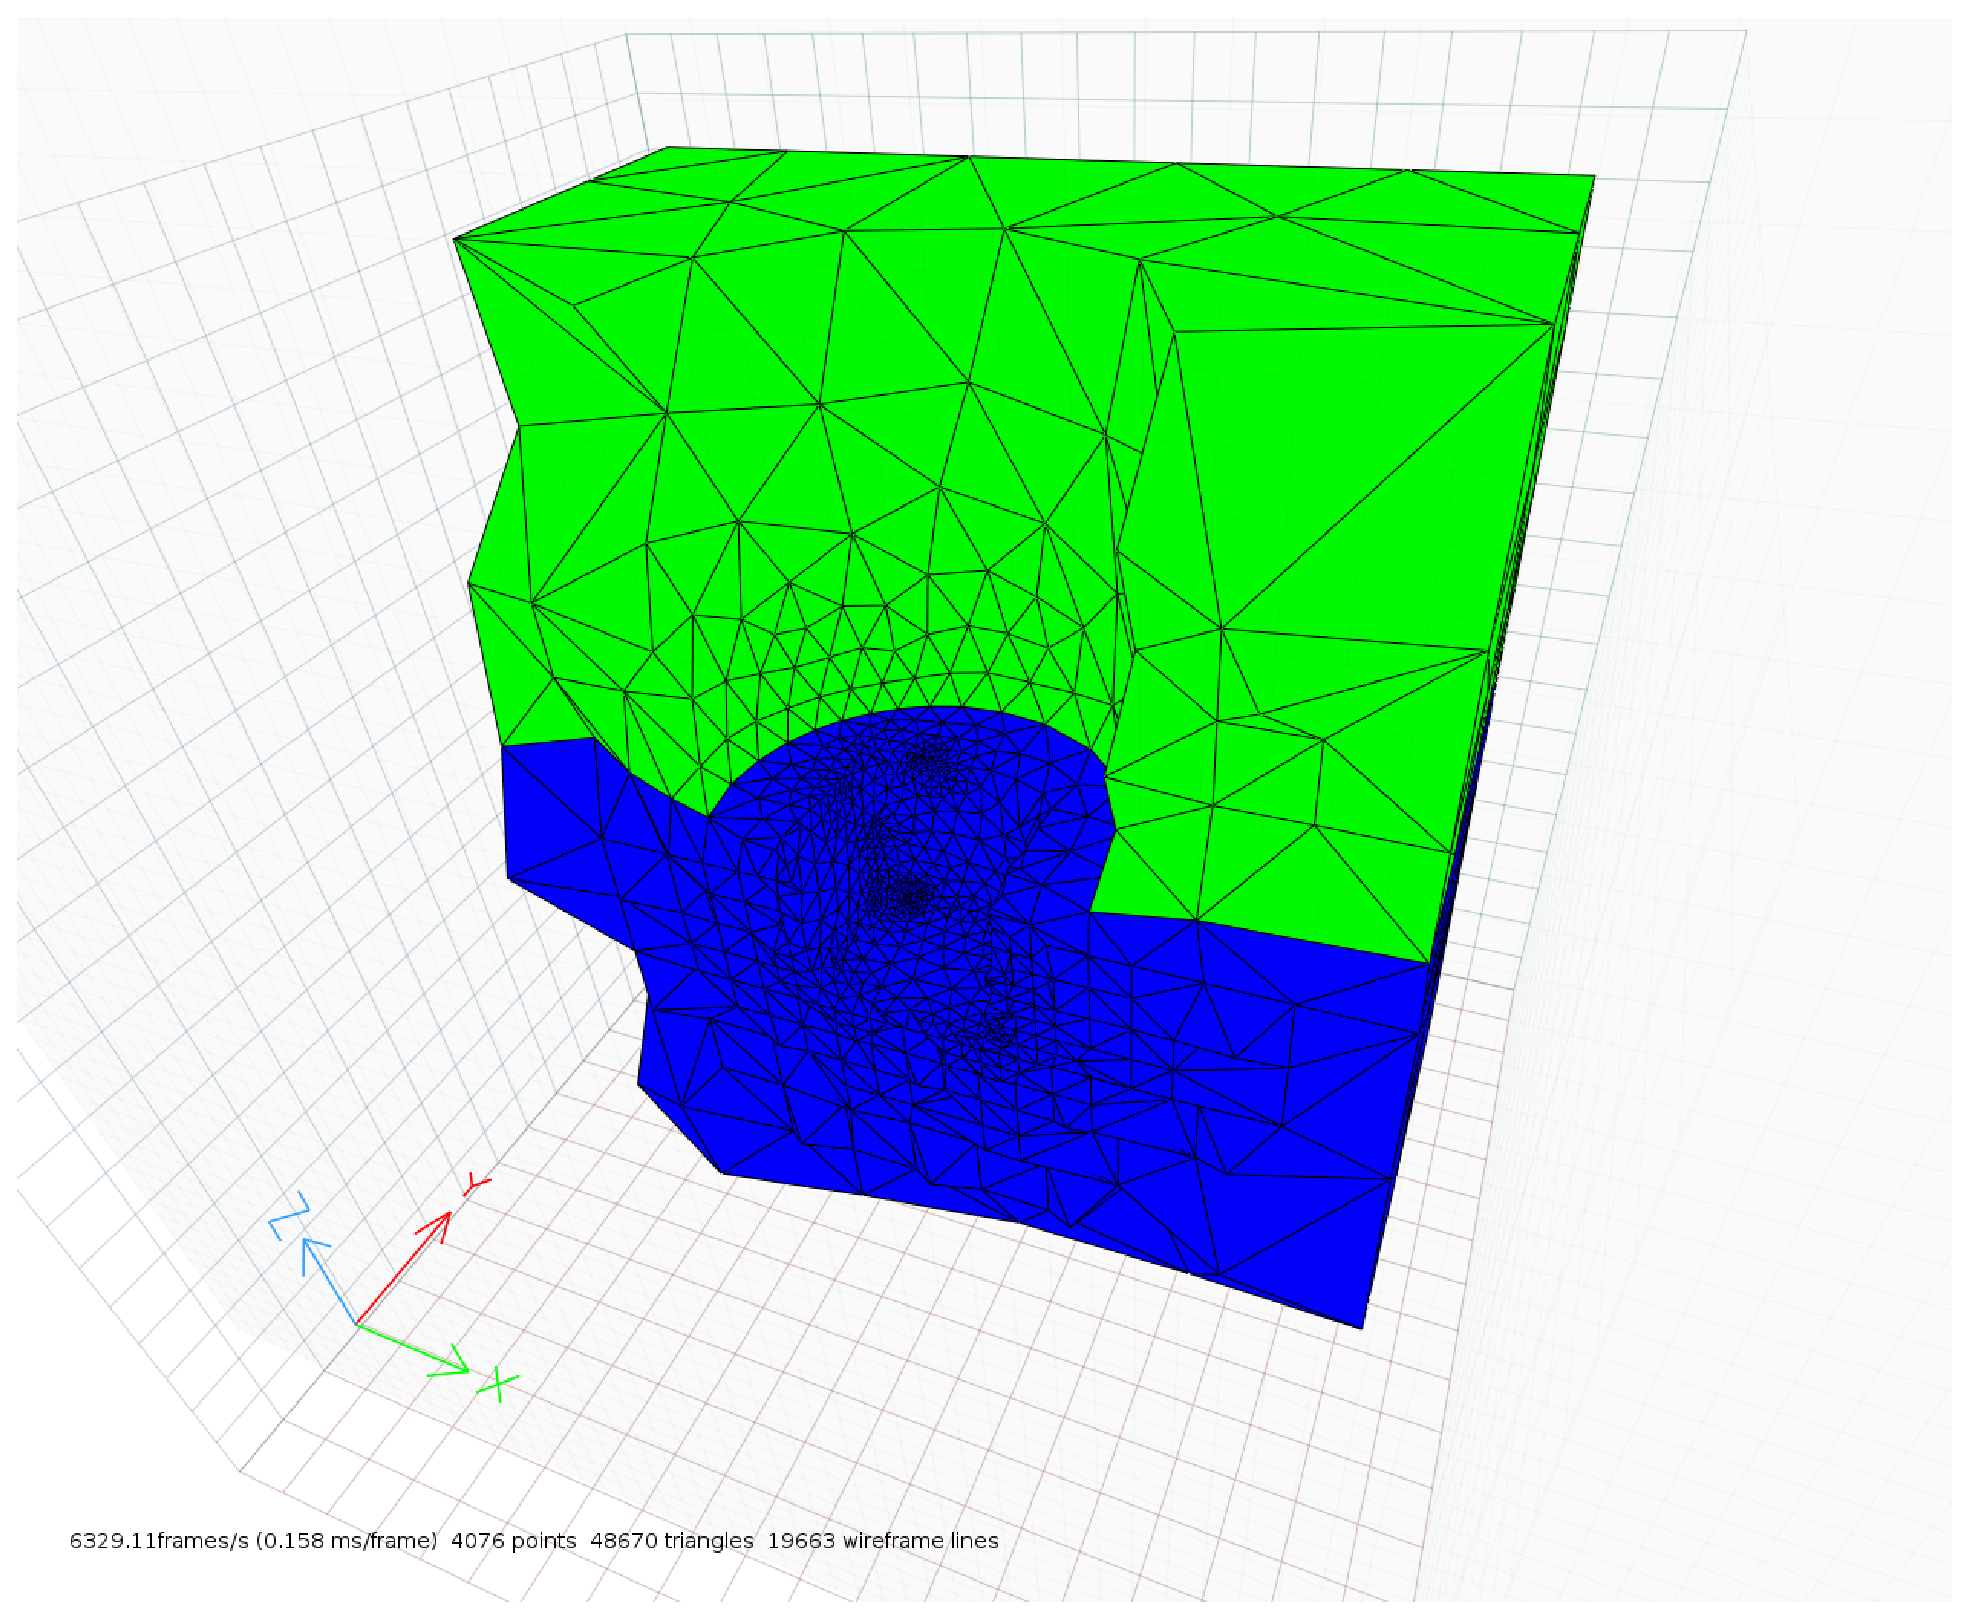
\includegraphics[scale=0.2]{figures/raw/cyl_mask_etched_flux_orig_cut.eps}}
   }
   \subfloat%[\textsc{Adapted Mesh}]
   {
      \fbox{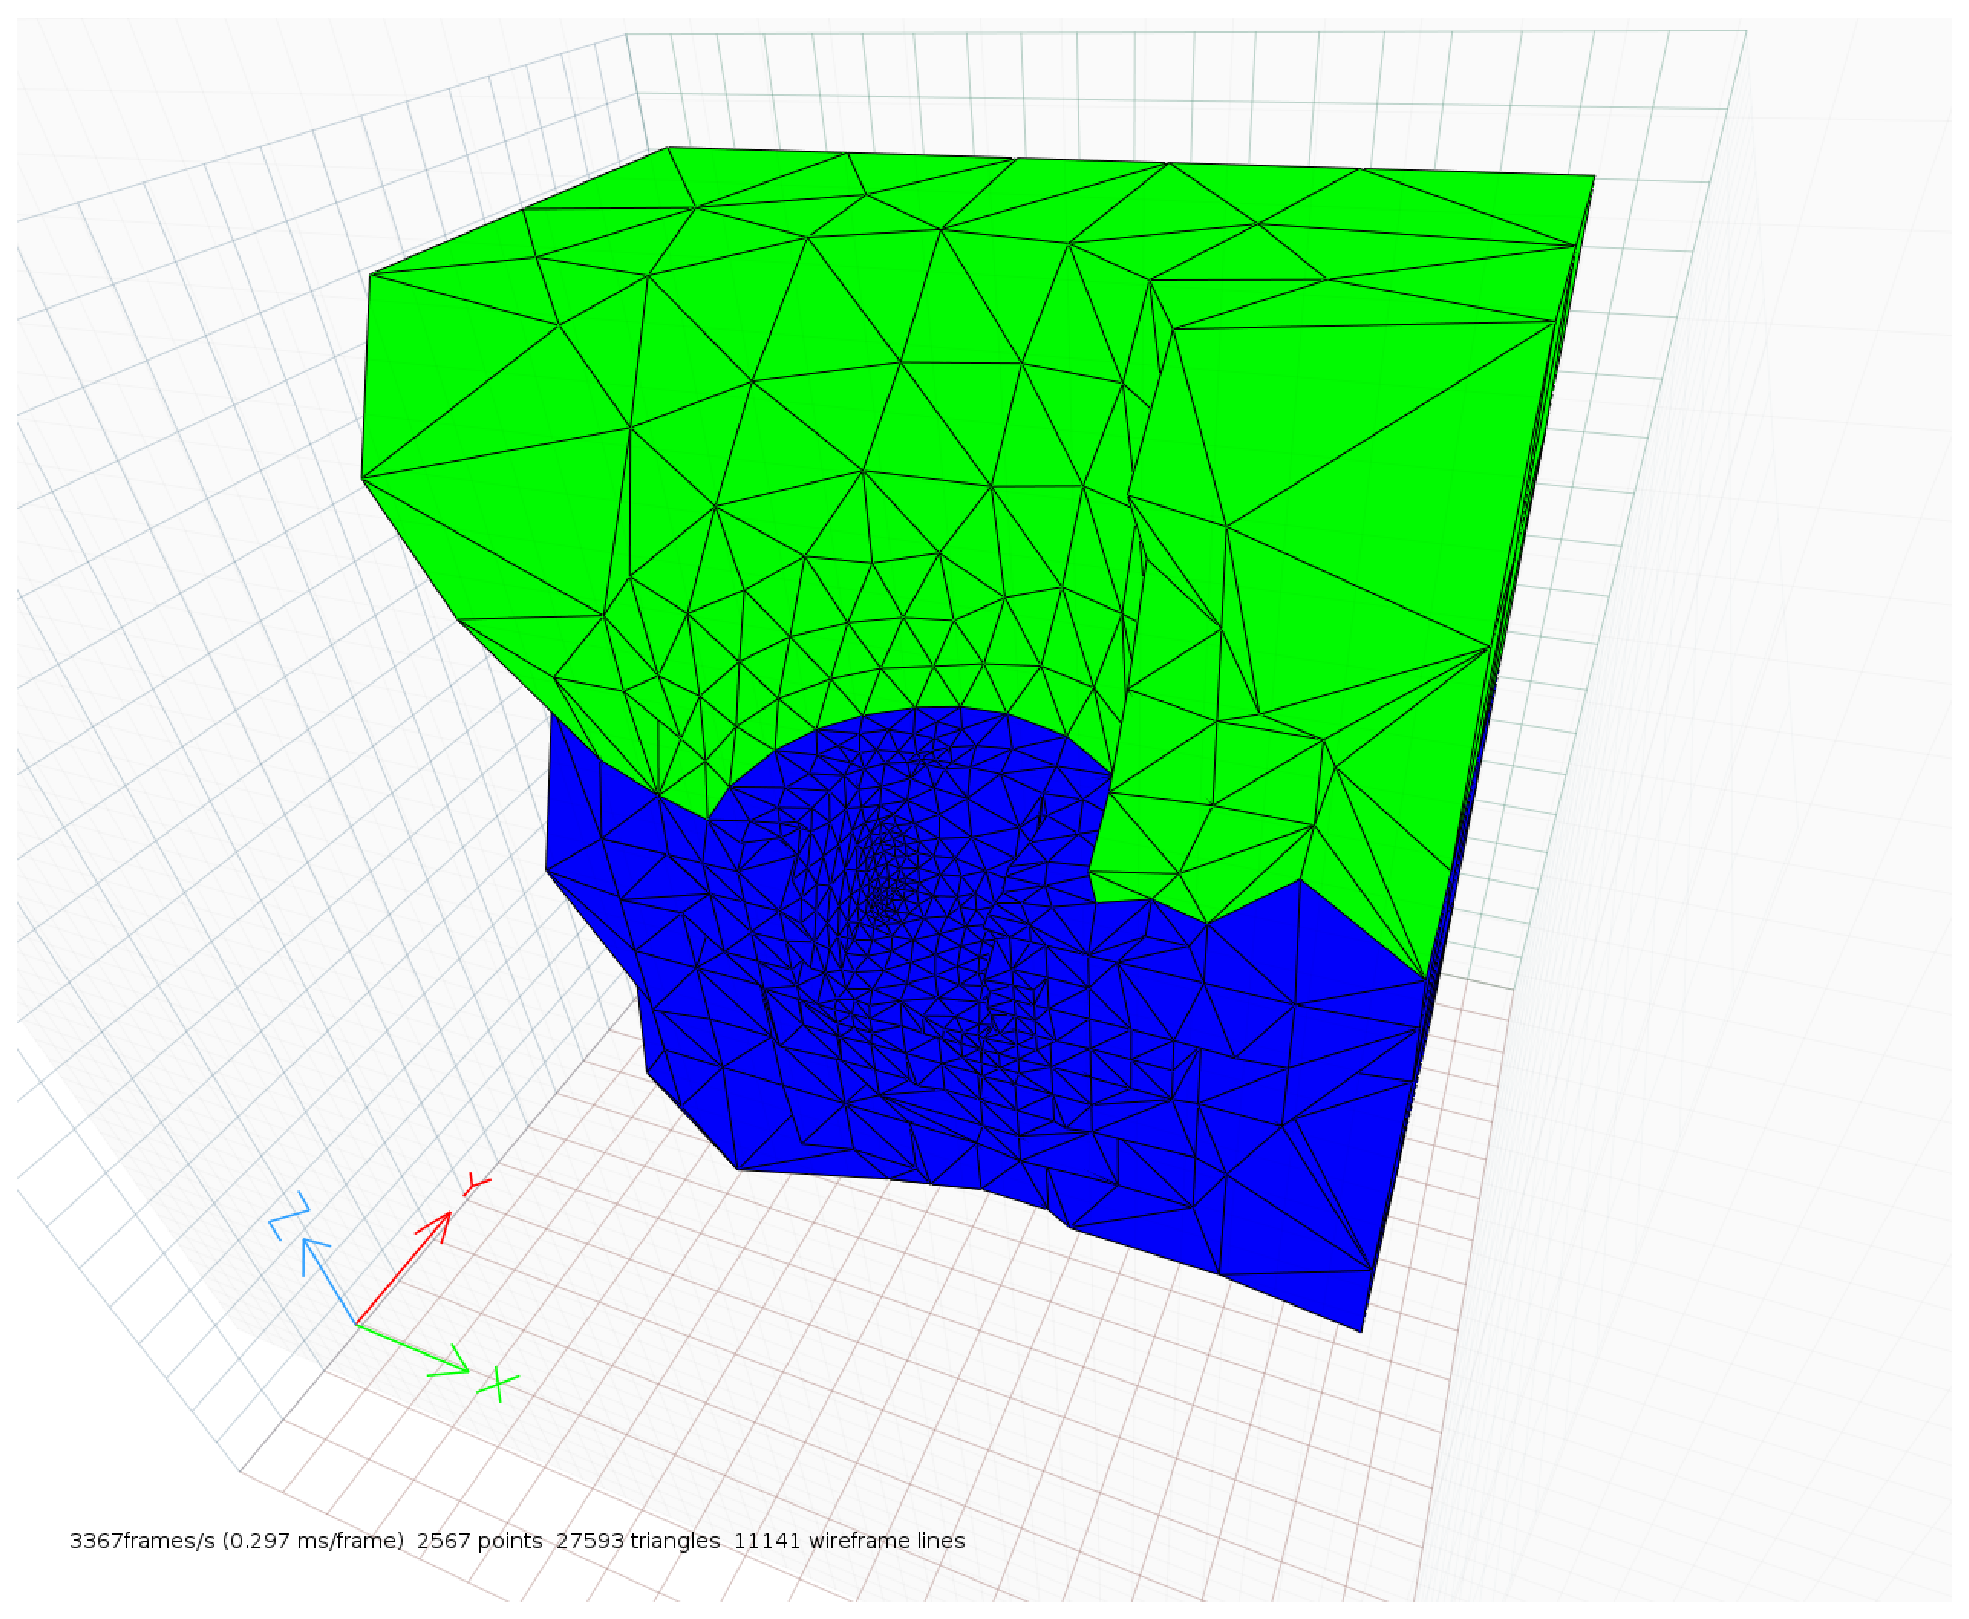
\includegraphics[scale=0.20]{figures/raw/cyl_mask_etched_flux_adapted_cut.eps}}
   }
   \caption{Etched hole with cylindrical mask.\newline  
   \textbf{left:} The initial mesh is shown. \textbf{right:} The adapted mesh is shown.}
\end{figure}

\begin{figure}[!ht]
   \centering

   \subfloat%[\textsc{Initial Mesh}]
   {
      \fbox{
      \begin{tabular}{ccc}
                           & \textbf{original} & \textbf{adapted} \\
      \hline 
      \textbf{vertex size} & 4076             & 2567 \\
      \end{tabular}
      }
   }

   \subfloat%[\textsc{Initial Mesh}]
   {
      \fbox{
      \begin{tabular}{crr}
      cap & 116 & 0.51\% \\
      needle & 290 & 1.27\% \\
      round & 18230 & 80.00\% \\
      slat & 728 & 3.19\% \\
      sliver & 1408 & 6.18\% \\
      spade & 283 & 1.24\% \\
      spindle & 96 & 0.42\% \\
      wedge & 1636 & 7.18\% \\
      \end{tabular}
      }
   }
   \subfloat%[\textsc{Adapted Mesh}]
   {
      \fbox{
      \begin{tabular}{crr}
      cap & 55 & 0.38\% \\
      needle & 169 & 1.18\% \\
      round & 11296 & 78.60\% \\
      slat & 483 & 3.36\% \\
      sliver & 964 & 6.71\% \\
      spade & 191 & 1.33\% \\
      spindle & 93 & 0.65\% \\
      wedge & 1121 & 7.80\% \\
      \end{tabular}
      }
   }

   \subfloat%[\textsc{Initial Mesh}]
   {
      \fbox{
      \setlength{\unitlength}{1cm}
      \psset{xunit=0.7cm, yunit=0.03017058cm}
      \begin{pspicture}(-1.0,-35.00000000)(10.66666667,130)
      \psaxes[labels=y,Dx=1,Dy=50.](0,0)(8,100)
      \pspolygon[fillcolor=black, fillstyle=solid](-0.08,104.55414013)(0,109.53290870)(0.08,104.55414013)
      \psframe[linewidth=1pt, fillcolor=gray, fillstyle=solid] (0.30000000,0)(0.70000000,0.51)
      \rput[bl](0.35000000,-35.00){\rotateleft{\footnotesize cap}}
      \psframe[linewidth=1pt, fillcolor=gray, fillstyle=solid] (1.30000000,0)(1.70000000,1.27)
      \rput[bl](1.35000000,-35.00){\rotateleft{\footnotesize needle}}
      \psframe[linewidth=1pt, fillcolor=gray, fillstyle=solid] (2.30000000,0)(2.70000000,80.00)
      \rput[bl](2.35000000,-35.00){\rotateleft{\footnotesize round}}
      \psframe[linewidth=1pt, fillcolor=gray, fillstyle=solid] (3.30000000,0)(3.70000000,3.19)
      \rput[bl](3.35000000,-35.00){\rotateleft{\footnotesize slat}}
      \psframe[linewidth=1pt, fillcolor=gray, fillstyle=solid] (4.30000000,0)(4.70000000,6.18)
      \rput[bl](4.35000000,-35.00){\rotateleft{\footnotesize sliver}}
      \psframe[linewidth=1pt, fillcolor=gray, fillstyle=solid] (5.30000000,0)(5.70000000,1.24)
      \rput[bl](5.35000000,-35.00){\rotateleft{\footnotesize spade}}
      \psframe[linewidth=1pt, fillcolor=gray, fillstyle=solid] (6.30000000,0)(6.70000000,0.42)
      \rput[bl](6.35000000,-35.00){\rotateleft{\footnotesize spindle}}
      \psframe[linewidth=1pt, fillcolor=gray, fillstyle=solid] (7.30000000,0)(7.70000000,7.18)
      \rput[bl](7.35000000,-35.00){\rotateleft{\footnotesize wedge}}
      \end{pspicture}

      }
   }
   \subfloat%[\textsc{Adapted Mesh}]
   {
      \fbox{
      \setlength{\unitlength}{1cm}
      \psset{xunit=0.7cm, yunit=0.03017058cm}
      \begin{pspicture}(-1.0,-35.00000000)(10.66666667,130)
      \psaxes[labels=y,Dx=1,Dy=50.](0,0)(8,100)
      \pspolygon[fillcolor=black, fillstyle=solid](-0.08,104.55414013)(0,109.53290870)(0.08,104.55414013)
      \psframe[linewidth=1pt, fillcolor=gray, fillstyle=solid] (0.30000000,0)(0.70000000,0.38)
      \rput[bl](0.35000000,-35.00){\rotateleft{\footnotesize cap}}
      \psframe[linewidth=1pt, fillcolor=gray, fillstyle=solid] (1.30000000,0)(1.70000000,1.18)
      \rput[bl](1.35000000,-35.00){\rotateleft{\footnotesize needle}}
      \psframe[linewidth=1pt, fillcolor=gray, fillstyle=solid] (2.30000000,0)(2.70000000,78.60)
      \rput[bl](2.35000000,-35.00){\rotateleft{\footnotesize round}}
      \psframe[linewidth=1pt, fillcolor=gray, fillstyle=solid] (3.30000000,0)(3.70000000,3.36)
      \rput[bl](3.35000000,-35.00){\rotateleft{\footnotesize slat}}
      \psframe[linewidth=1pt, fillcolor=gray, fillstyle=solid] (4.30000000,0)(4.70000000,6.71)
      \rput[bl](4.35000000,-35.00){\rotateleft{\footnotesize sliver}}
      \psframe[linewidth=1pt, fillcolor=gray, fillstyle=solid] (5.30000000,0)(5.70000000,1.33)
      \rput[bl](5.35000000,-35.00){\rotateleft{\footnotesize spade}}
      \psframe[linewidth=1pt, fillcolor=gray, fillstyle=solid] (6.30000000,0)(6.70000000,0.65)
      \rput[bl](6.35000000,-35.00){\rotateleft{\footnotesize spindle}}
      \psframe[linewidth=1pt, fillcolor=gray, fillstyle=solid] (7.30000000,0)(7.70000000,7.80)
      \rput[bl](7.35000000,-35.00){\rotateleft{\footnotesize wedge}}
      \end{pspicture}
      }
   }
   \caption{A mesh quality analysis of the original and the adapted etched hole meshes. 
   The analysis of the initial mesh and the adapted mesh is depicted, on the \textbf{left}
   \textbf{right}, respectively. Apparently, the mesh adaption process 
   introduces a bit more \texttt{slivers}, on the other hand, a significant amount 
   of rounds is introduced too. The mesh elements remained more or less the same, however, 
   the mesh vertex size is again considerably decreased.}
\end{figure}


